%!TEX root = widefieldscan.tex
\svnidlong
{$HeadURL$}
{$LastChangedDate$}
{$LastChangedRevision$}
{$LastChangedBy$}

\ifhtml
\else
\begin{center}
	\fbox{
		\begin{minipage}{.618\columnwidth}
		The section below is versioned at \url{\svnkw{HeadURL}} (last commit @ \svnfileday.\svnfilemonth.\svnfileyear \space \svnfilehour:\svnfileminute, Revision: \svnkw{LastChangedRevision}).
		\end{minipage}
	} 
\end{center}
\fi

\section{Results}%
\label{sec:Results}%
\subsection{Image Merging and Reconstruction}%
\label{sec:Image Merging and Reconstruction}%
Multiple independently acquired projection images covering the desired field of view have been merged into single projections covering the full field of view. Figure~\ref{fig:subscans} shows exemplary projection images from overlapping subscans prior to correction and normalization. Figure~\ref{fig:merge-proj} shows a merged projection image prior to reconstruction and figure~\ref{fig:merge-rec} shows one slice of the reconstructed dataset acquired from 5244 projections. Such a reconstructed slice covers a field of view of \SI{2792}{pixels} (\SI{4.13}{\milli\meter}) which is three times the size of what can be achieved with one single binned scan (\SI{1024}{pixels} or \SI{1.52}{\milli\meter}). %1024 * 1.48 um/px = 1.51552mm

\ifiucr
	%\onecolumn
	\begin{figure}%
		\caption{Wide field scan of a rat lung sample obtained from a Sprague-Dawley rat 21 days after birth, showing the distal-medial edge of the right lower lung lobe. The sample has been scanned at \SI{12.6}{\kilo\electronvolt}, the protocol details conform to protocol ``B'', described in table~\ref{tab:protocols}. %
		a) Three uncorrected and independent projection images from subscans s$_1$--s$_3$, each with a size of 1024\(\times\)1024 pixels at a resolution of \SI{1.48}{\micro\meter\per pixel}, each covering a field of view of \SI{1.52}{\milli\meter}. Subscans s$_1$ and s$_2$ overlap each other by 141 pixels (red and green overlay), subscans s$_2$ and s$_3$ overlap each other by 138 pixels (blue and yellow overlay). 5244 projections  over a rotation of \SI{180}{\degree} have been acquired for all subscans. %
		b) Merged and corrected image from the three subscans shown in subfigure a). Each merged projection has a size of 2793\(\times\)1024 pixels at a resolution of \SI{1.48}{\micro\meter\per pixel}. The width of the merged projections is slightly smaller than three times the width of the subscans due to the overlap needed to merge the projections (2793~px$=3\cdot3072$~px$-141$~px$-138$~px). Since the x-ray beam is extremely stable, the bands visible in the raw projections can be eliminated. %
		c) Cropped part of one slice of the tomographic dataset reconstructed from 5244 merged projections shown in subfigure b). Due to the coherence of the x-ray beam the air-to-paraffin interface is visible around the sample.%
		}%
		\label{fig:wide field scan results}%
		%\documentclass{article}
%\usepackage{subfig}
%\usepackage{tikz}
%\usepackage{siunitx}
%\begin{document}
%\newcommand{\imsize}{\linewidth}
%\newlength\imagewidth % needed for scalebars
%\newlength\imagescale % needed for scalebars
%\begin{figure}
%	\centering
%%%%%%%%%%%%%%%%%%%%%%%%%%%%%
	\renewcommand{\imsize}{.333\linewidth}
	\pgfmathsetlength{\imagewidth}{\imsize} % desired display width of image
	\pgfmathsetlength{\imagescale}{\imagewidth/1024} % pixel width of image
			% --------------------------------------------------------------
			% Cutline between SubScan 1 and 2: 141 pixels
			% Cutline between SubScan 2 and 3: 138 pixels
			% --------------------------------------------------------------
			\def\size{1023}%
			\begin{tikzpicture}[x=\imagescale,y=-\imagescale]%
				\node[anchor=north west, inner sep=0pt, outer sep=0pt] at (0,0)%
					{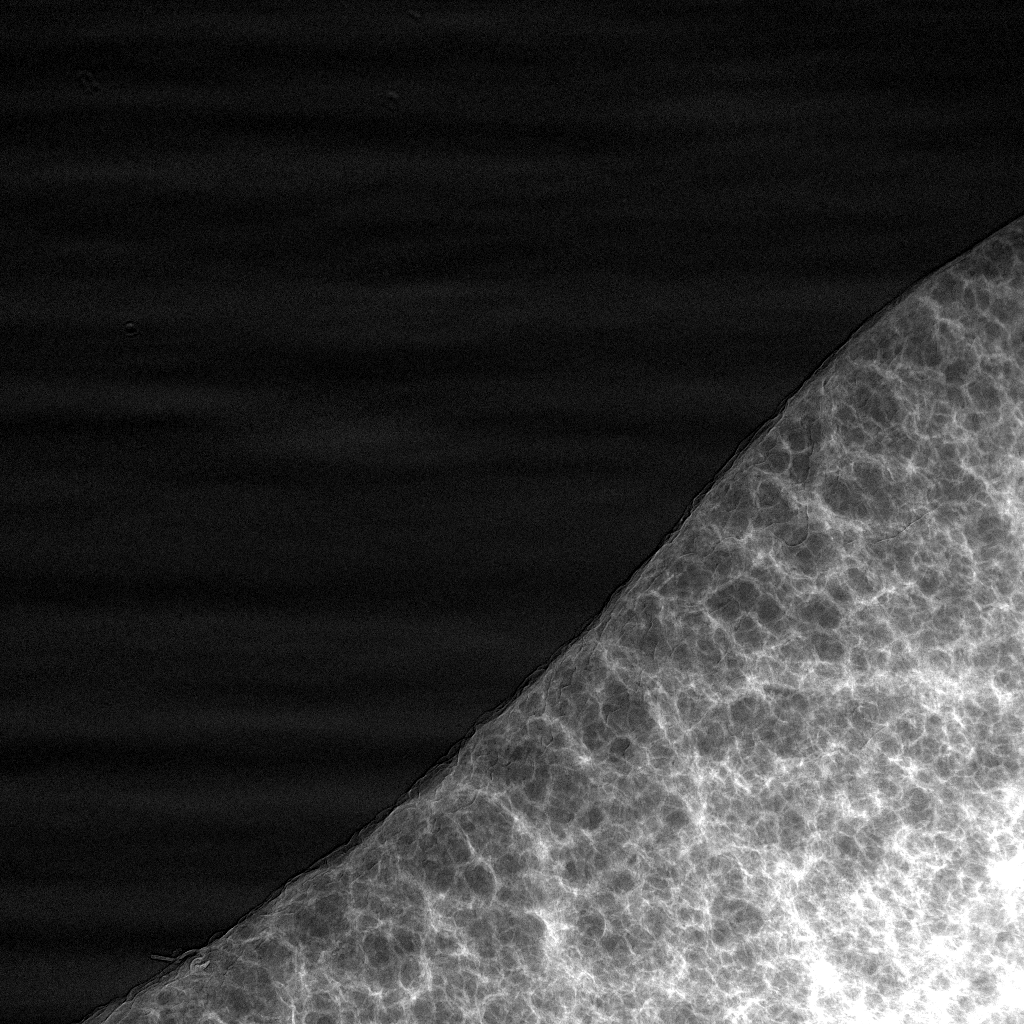
\includegraphics[width=\imagewidth]{img/merge/CP-R108C21Cb_s13358_normalize}};%
%					{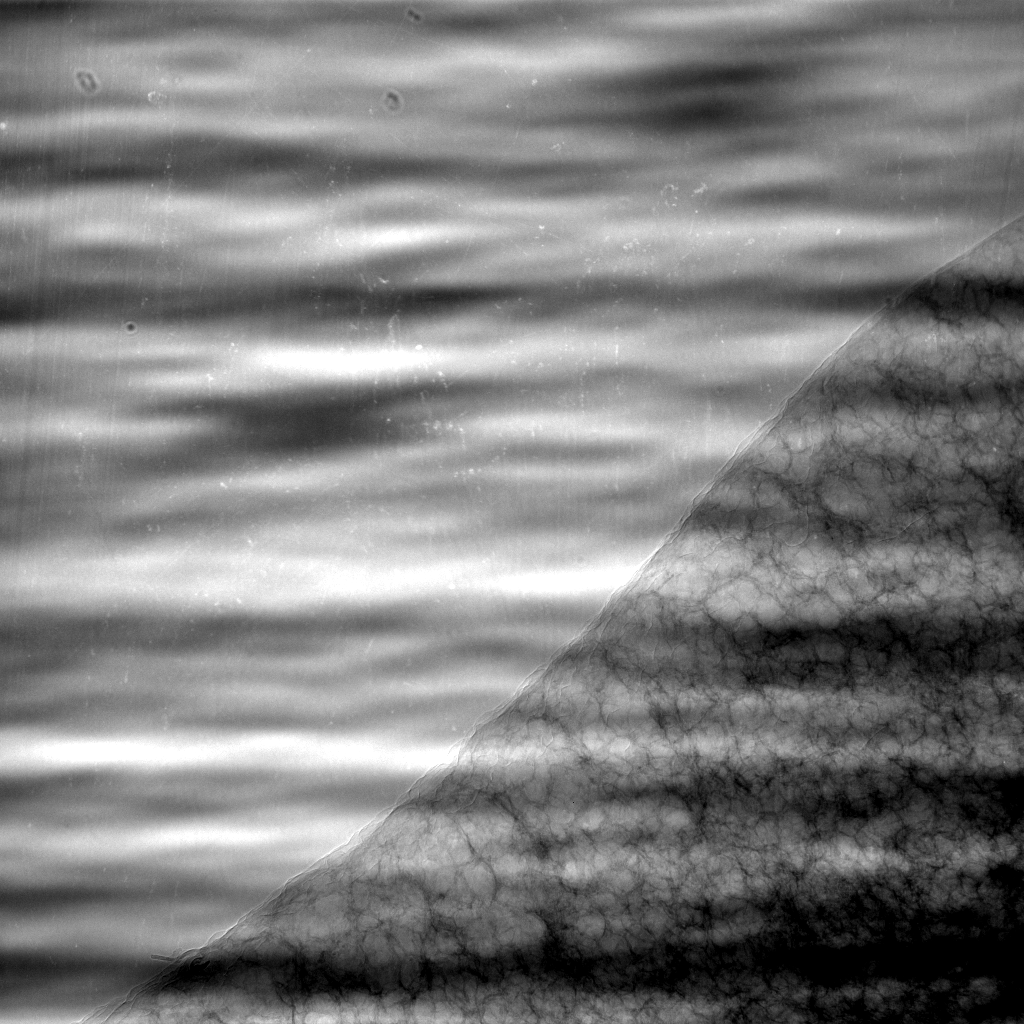
\includegraphics[width=\imagewidth]{R108C21Cb_s13358_normalize}};%
				\def\overlap{141}%
				\fill [red, nearly transparent] (1024-\overlap,1) rectangle (\size,\size);%
				\draw (1024-\overlap,1) rectangle (\size,\size);%
				\node [anchor=south west, color=white] at (0,1024) {(a)};				
			\end{tikzpicture}%
			\begin{tikzpicture}[x=\imagescale,y=-\imagescale]%
				\node[anchor=north west, inner sep=0pt, outer sep=0pt] at (0,0)%
					{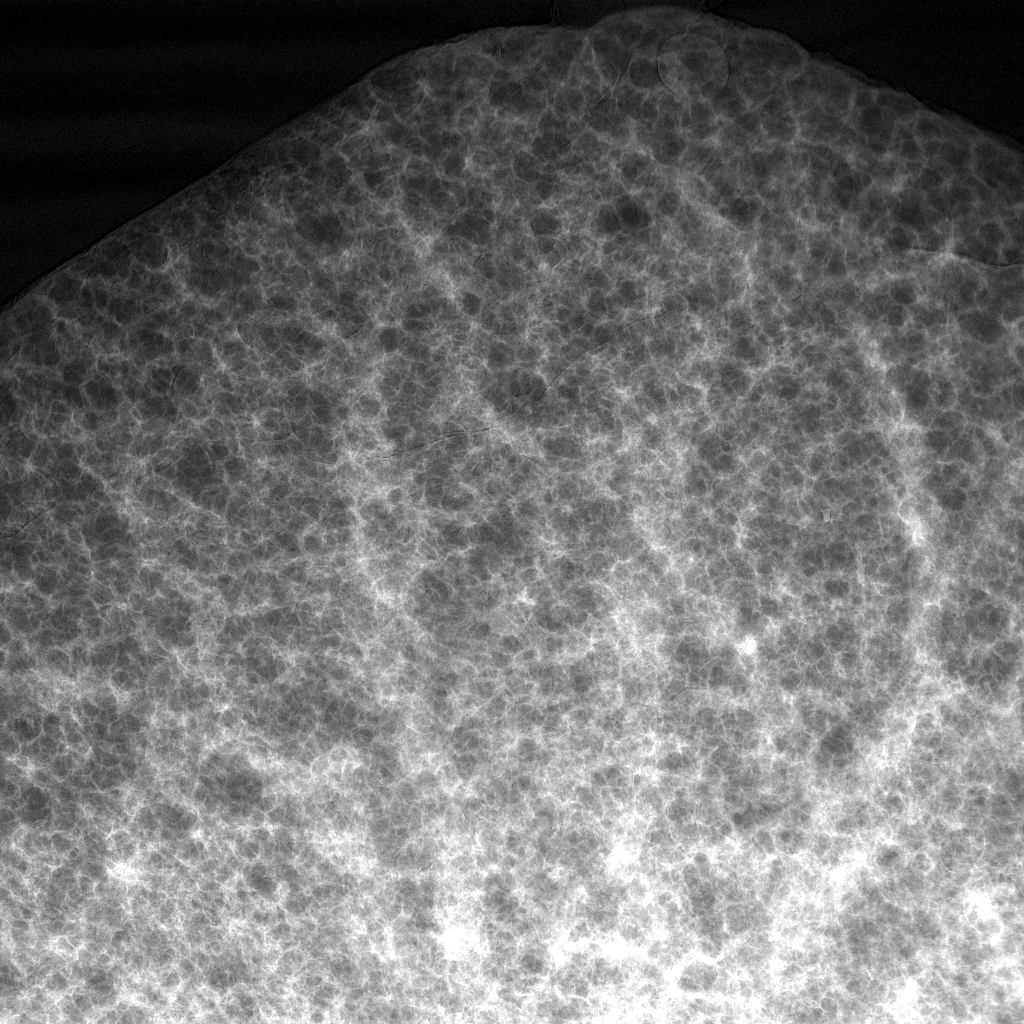
\includegraphics[width=\imagewidth]{img/merge/CP-R108C21Cb_s23358_normalize}};%
%					{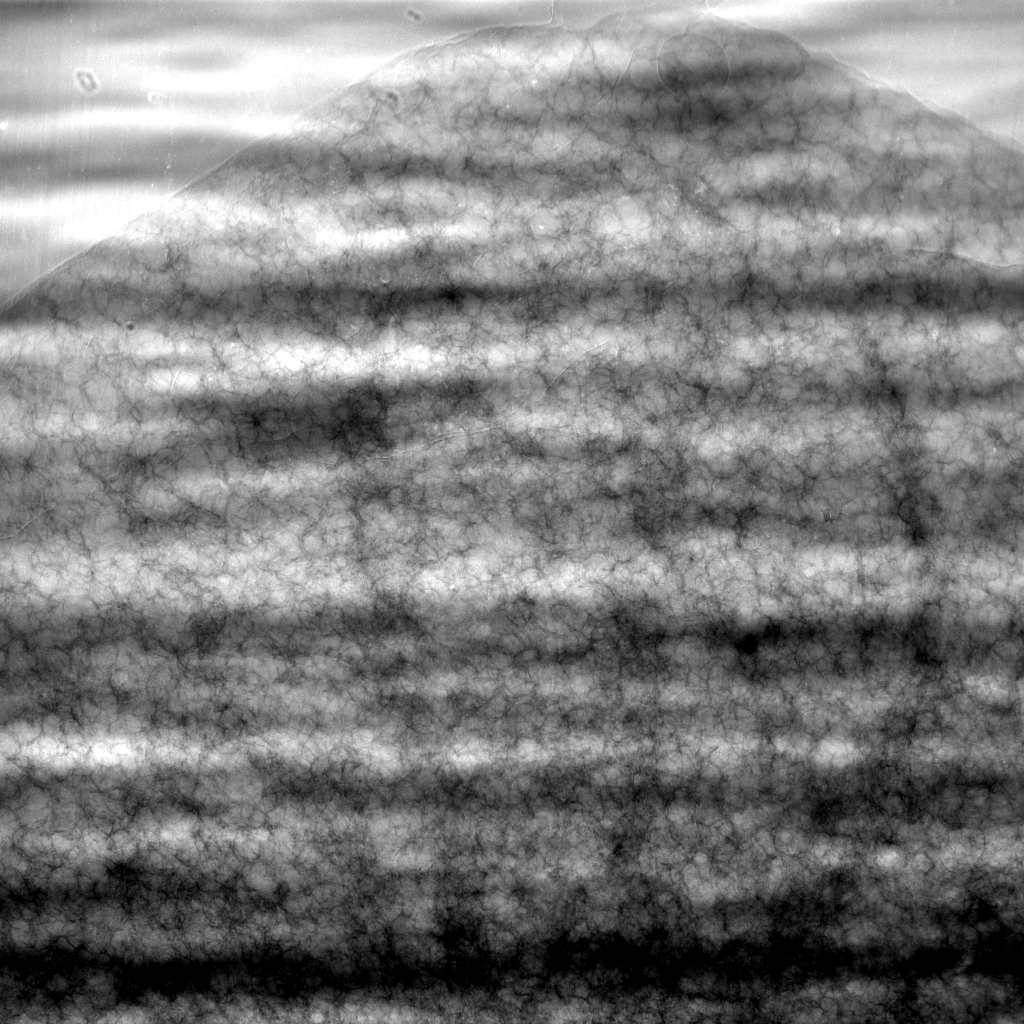
\includegraphics[width=\imagewidth]{R108C21Cb_s23358_normalize}};%
				\def\overlap{141}%
				\fill [green, nearly transparent] (1,1) rectangle (\overlap,\size);%
				\draw (1,1) rectangle (\overlap,\size);%
				\def\overlap{138}%
				\fill [blue, nearly transparent] (1024-\overlap,1) rectangle (\size,\size);%
				\draw (1024-\overlap,1) rectangle (\size,\size);%
			\end{tikzpicture}%
			\begin{tikzpicture}[x=\imagescale,y=-\imagescale]%
				% place image (integer coordinates refer to pixel centers):
				\node[anchor=north west, inner sep=0pt, outer sep=0pt] at (0,0)%
					{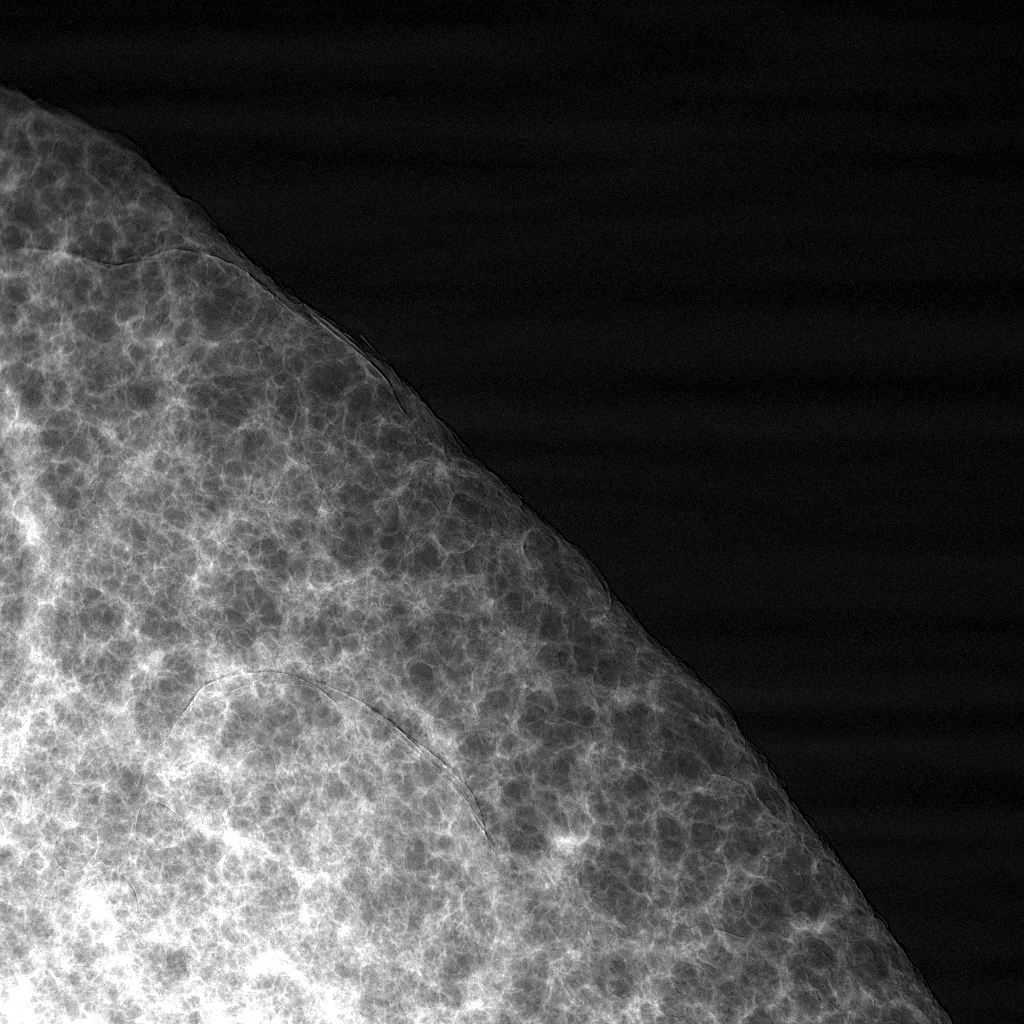
\includegraphics[width=\imagewidth]{img/merge/CP-R108C21Cb_s33358_normalize}};%
%					{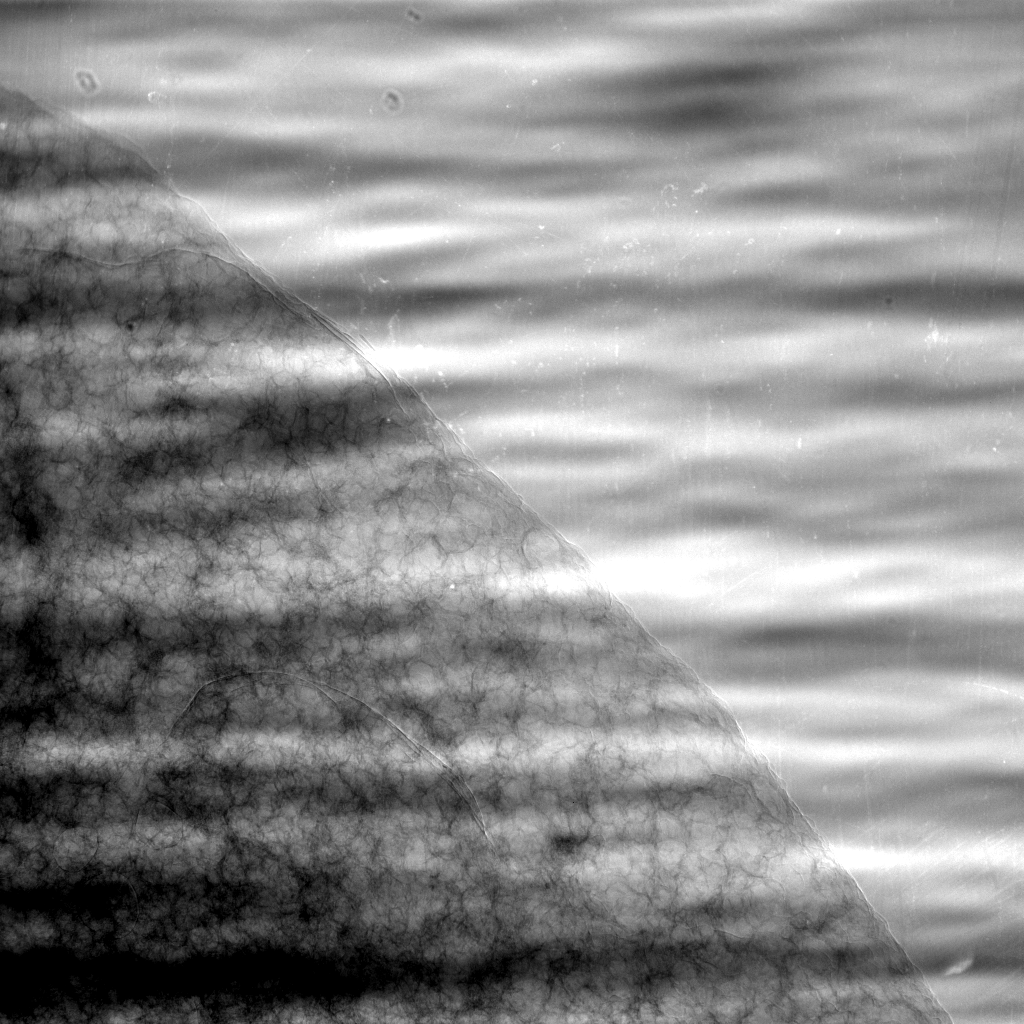
\includegraphics[width=\imagewidth]{R108C21Cb_s33358_normalize}};%
				\def\overlap{138}%
				\fill [yellow, nearly transparent] (1,1) rectangle (\overlap,\size);%
				\draw (1,1) rectangle (\overlap,\size);%
%				\draw[|-|,thick] (5,200) -- (1021,200) node [color=white,midway,above] {\SI{1.51552}{\milli\meter}};%
				\def\x{924}% 1024 - 100
				\def\y{922}% 1024 * .9 = 921.6
				\def\bar{338}% 100 px = 148 um
				\draw[|-|,thick, color=white] (\x-\bar,\y) -- (\x,\y) node [midway, above] {\SI{500}{\micro\meter}};%
			\end{tikzpicture}%
			\label{fig:subscans}%
%%%%%%%%%%%%%%%%%%%%%%%%%%%%%	
%	\caption{caption}
%\end{figure}
%\end{document}\\%
		%\documentclass{article}
%\usepackage{subfig}
%\usepackage{tikz}
%\usepackage{siunitx}
%\begin{document}
%\newcommand{\imsize}{\linewidth}
%\newlength\imagewidth % needed for scalebars
%\newlength\imagescale % needed for scalebars
%\begin{figure}
%	\centering
%%%%%%%%%%%%%%%%%%%%%%%%%%%%%
		\renewcommand{\imsize}{\linewidth}%
		\pgfmathsetlength{\imagewidth}{\imsize} % desired displayed width of image
		\pgfmathsetlength{\imagescale}{\imagewidth/2793}% pixel width of image
			\begin{tikzpicture}[x=\imagescale,y=-\imagescale]%
				\node[anchor=north west,inner sep=0pt,outer sep=0pt] at (0,0)%
					{\includegraphics[width=\imagewidth]{img/merge/R108C21Cb_mrg3333_normalize}};%
%					{\includegraphics[width=\imagewidth]{R108C21Cb_mrg3333_normalize}};%
				\def\x{2693} % 2793-100
				\def\y{922} % 1024*.9 = 921.6
				\def\bar{338} % 100 px = 148 um
				\draw[|-|,thick,color=white] (5,256) -- (2787,256) node [midway,above] {\SI{4.13364}{\milli\meter}};
				\draw[|-|,thick,color=white] (\x-\bar,\y) -- (\x,\y) node [midway,above] {\SI{500}{\micro\meter}};
				\node [anchor=center,color=white] at (100,1024-100) {b)};
				\end{tikzpicture}%
			\label{fig:merge-proj}%
%%%%%%%%%%%%%%%%%%%%%%%%%%%%%	
%	\caption{caption}
%\end{figure}
%\end{document}\\%
		%\documentclass{article}
%\usepackage{subfig}
%\usepackage{tikz}
%\usepackage{siunitx}
%\begin{document}
%\newcommand{\imsize}{\linewidth}
%\newlength\imagewidth % needed for scalebars
%\newlength\imagescale % needed for scalebars
%\begin{figure}
%	\centering
%%%%%%%%%%%%%%%%%%%%%%%%%%%%%
		\pgfmathsetlength{\imagewidth}{\imsize}%
		\pgfmathsetlength{\imagescale}{\imagewidth/2792}%
			\begin{tikzpicture}[x=\imagescale,y=-\imagescale]%
				\node [anchor=north west,inner sep=0pt,outer sep=0pt] at (0,0)%
					{\includegraphics[width=\imagewidth]{img/merge/R108C21Cb_mrg1024rec8bit}};% ``mogrify -shave 0x900 -format png R108C21Cb_mrg1024rec8bit.tif''
%					{\includegraphics[width=\imagewidth]{R108C21Cb_mrg1024rec8bit}};
				\clip (0,0) rectangle (2792,992);				
				\def\x{2692} % 2792-100
				\def\y{893} % 992 * .9 = 892.8
				\def\bar{338} % 100 px = 148 um
				%%%% scalebar
					\draw[|-|,thick,color=white] (\x-\bar,\y) -- (\x,\y) node [midway, above] {\SI{500}{\micro\meter}};
%					\draw[|-|,thick,color=white] (5,30) -- (2787,30) node [midway, below] {\SI{4.13216}{\milli\meter}};
				%%%% center
					\fill [color=red] (2792/2,992/2) circle (5);
				%%%% big circle
					\draw [dashed, ultra thick, color=red] (2792/2,992/2) circle (512);
					\def\angle{35}
					\draw [white, thick, <->] (2792/2,992/2) +(\angle:0) --  node (bigto) {} +(\angle:512); 
					\node [white] (bigfrom) at (349,256){$\frac{1024}{2}$px};
					\draw [white, ->, thick, densely dotted] (bigfrom) to [bend left=45] (bigto);
				%%%% big circle
				%%%% 141px circle
				\draw [dashed, ultra thick, color=red] (2792/2,992/2) circle (512-141);
				\def\angle{35+90}
					\draw [white,thick,<->] (2792/2,992/2) +(\angle:0) -- node (smallto) {} +(\angle:512-141);
					\node [white] (smallfrom) at (349,384) {$\frac{1024}{2}-141$px};
					\draw [white, ->, thick, densely dotted] (smallfrom) to [bend left=45] (smallto);
				%%%% 141px circle					
%				%%%% 138px circle
%				\draw [dashed,color=red] (2792/2,992/2) circle (512-138);
%				\def\angle{45+90+90}
%					\draw [white,<->] (2792/2,992/2) +(\angle:0) -- node (vsmallto) {} +(\angle:512-138);
%					\node [white] (vsmallfrom) at (2972-768,992-512) {$\frac{1024}{2}-138$px};
%					\draw [white,->,densely dotted] (vsmallfrom) to [bend right=45] (vsmallto);
%				%%%% 138px circle
				%%%% inset
%				\newcommand{\size}{.2\imagewidth}%
%				\clip (256,256) rectangle (512,512);
%				\node[anchor=north west,inner sep=0pt,outer sep=0pt] at (0,0)
%					{\includegraphics[width=\size]{R108C21Cb_mrg1024rec8bit}};
%					\draw[white] (0,0) rectangle (\size,-\size);
				%%%% inset
				\node [anchor=south west, color=white] at (0,990) {(c)};			
				\end{tikzpicture}%
			\label{fig:merge-rec}%
%%%%%%%%%%%%%%%%%%%%%%%%%%%%%	
%	\caption{caption}
%\end{figure}
%\end{document}\\%
	\end{figure}%
	%\twocolumn
\else
	\begin{figure*}[htp]
		%\documentclass{article}
%\usepackage{subfig}
%\usepackage{tikz}
%\usepackage{siunitx}
%\begin{document}
%\newcommand{\imsize}{\linewidth}
%\newlength\imagewidth % needed for scalebars
%\newlength\imagescale % needed for scalebars
%\begin{figure}
%	\centering
%%%%%%%%%%%%%%%%%%%%%%%%%%%%%
	\renewcommand{\imsize}{.33\linewidth}
	\pgfmathsetlength{\imagewidth}{\imsize} % desired display width of image
	\pgfmathsetlength{\imagescale}{\imagewidth/1024} % pixel width of image
	\centering
		\subfloat[Three uncorrected and independent projection images from subscans s$_1$--s$_3$, each with a size of 1024\(\times\)1024 pixels at a resolution of \SI{1.48}{\micro\meter\per pixel}, each covering a FOV of \SI{1.52}{\milli\meter}. Subscans s$_1$ and s$_2$ overlap each other by 141 pixels (red and green overlay), subscans s$_2$ and s$_3$ overlap each other by 138 pixels (blue and yellow overlay). 5244 projections  over a rotation of \SI{180}{\degree} have been acquired for all subscans.]{%
			\label{fig:s1}%
			% --------------------------------------------------------------
			% Cutline between SubScan 1 and 2: 141 pixels
			% Cutline between SubScan 2 and 3: 138 pixels
			% --------------------------------------------------------------
			\begin{tikzpicture}[x=\imagescale,y=-\imagescale]%
				\node[anchor=north west,inner sep=0pt,outer sep=0pt] at (0,0)%
					{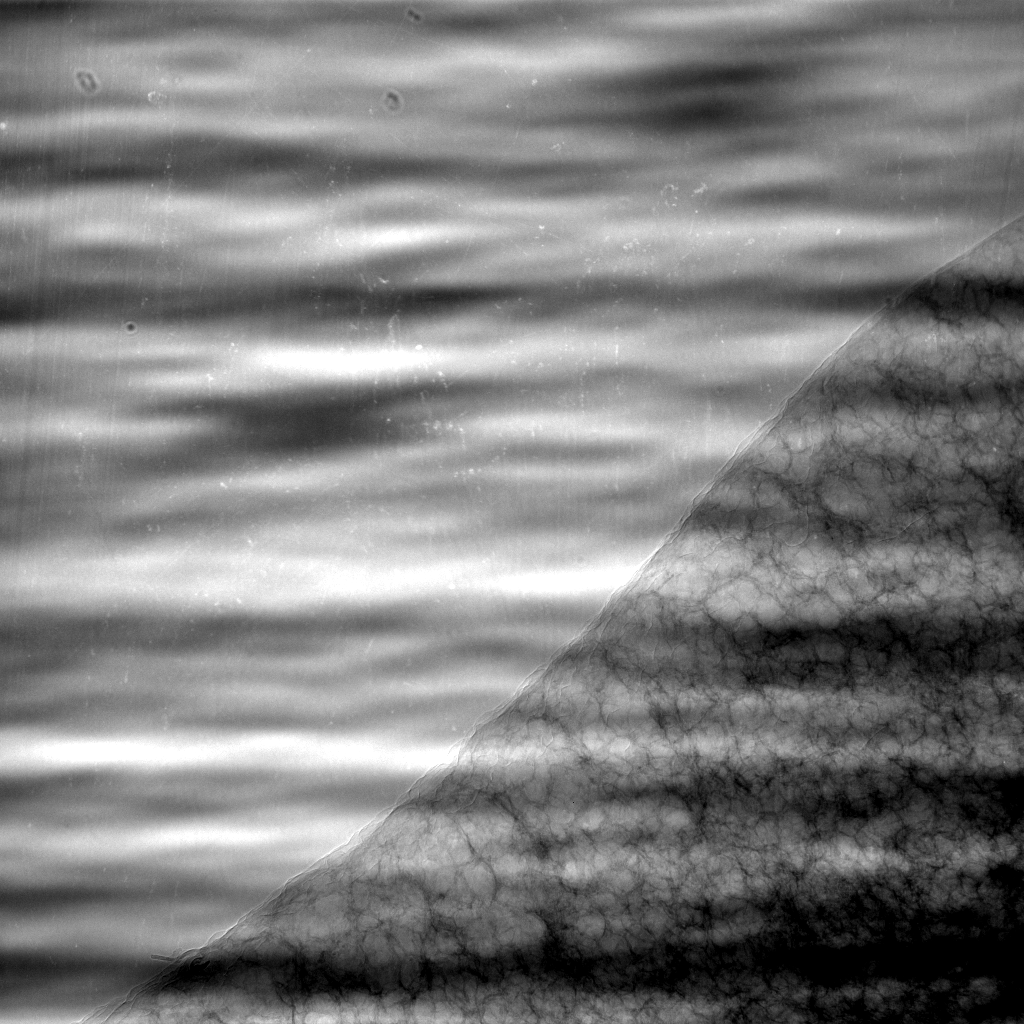
\includegraphics[width=\imagewidth]{R108C21Cb_s13358_normalize}};%
				\def\overlap{141}%
				\fill [red, nearly transparent] (1024-\overlap,1) rectangle (1024,1024);%
				\draw (1024-\overlap,1) rectangle (1024,1024);%
			\end{tikzpicture}%
			\begin{tikzpicture}[x=\imagescale,y=-\imagescale]%
				\node[anchor=north west,inner sep=0pt,outer sep=0pt] at (0,0)%
					{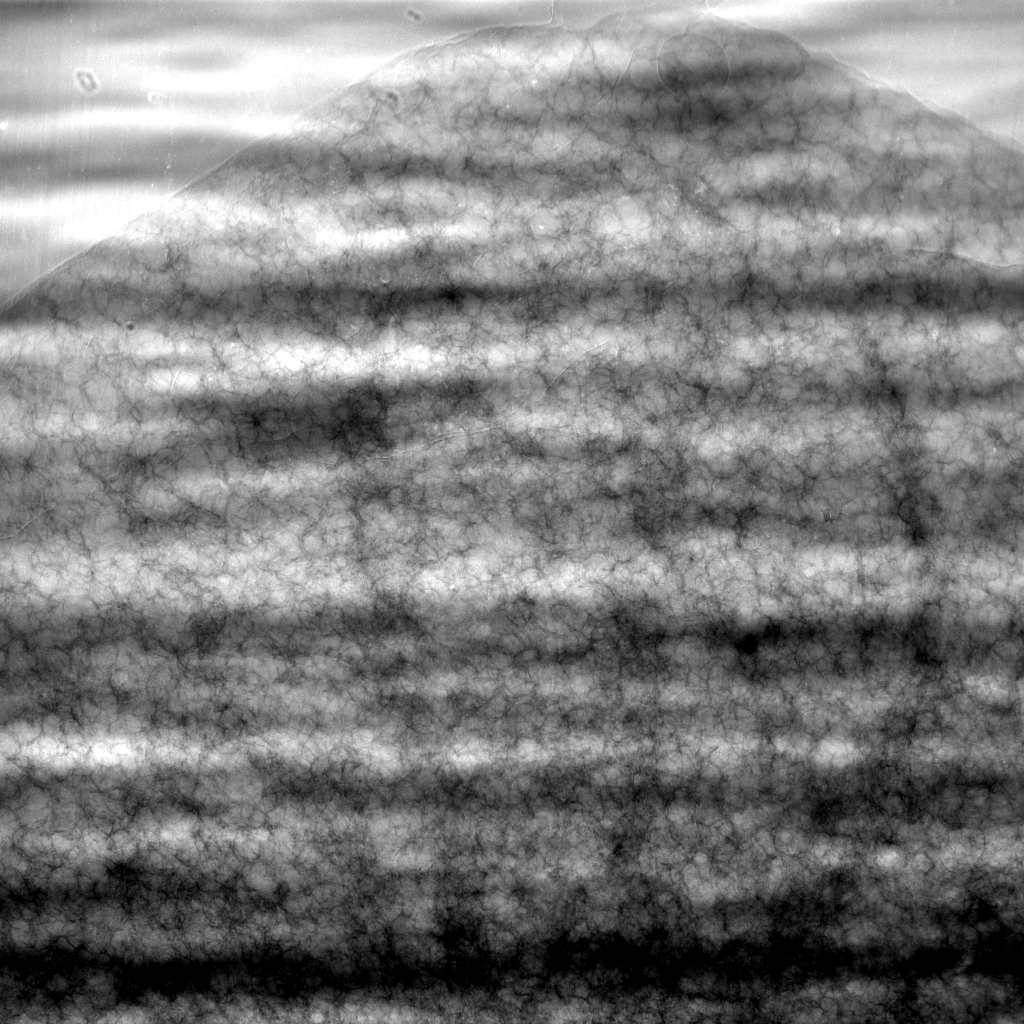
\includegraphics[width=\imagewidth]{R108C21Cb_s23358_normalize}};%
				\def\overlap{141}%
				\fill [green, nearly transparent] (1,1) rectangle (\overlap,1024);%
				\draw (1,1) rectangle (\overlap,1024);%
				\def\overlap{138}%
				\fill [blue, nearly transparent] (1024-\overlap,1) rectangle (1024,1024);%
				\draw (1024-\overlap,1) rectangle (1024,1024);%
			\end{tikzpicture}%
			\begin{tikzpicture}[x=\imagescale,y=-\imagescale]%
				% place image (integer coordinates refer to pixel centers):
				\node[anchor=north west,inner sep=0pt,outer sep=0pt] at (0,0)%
					{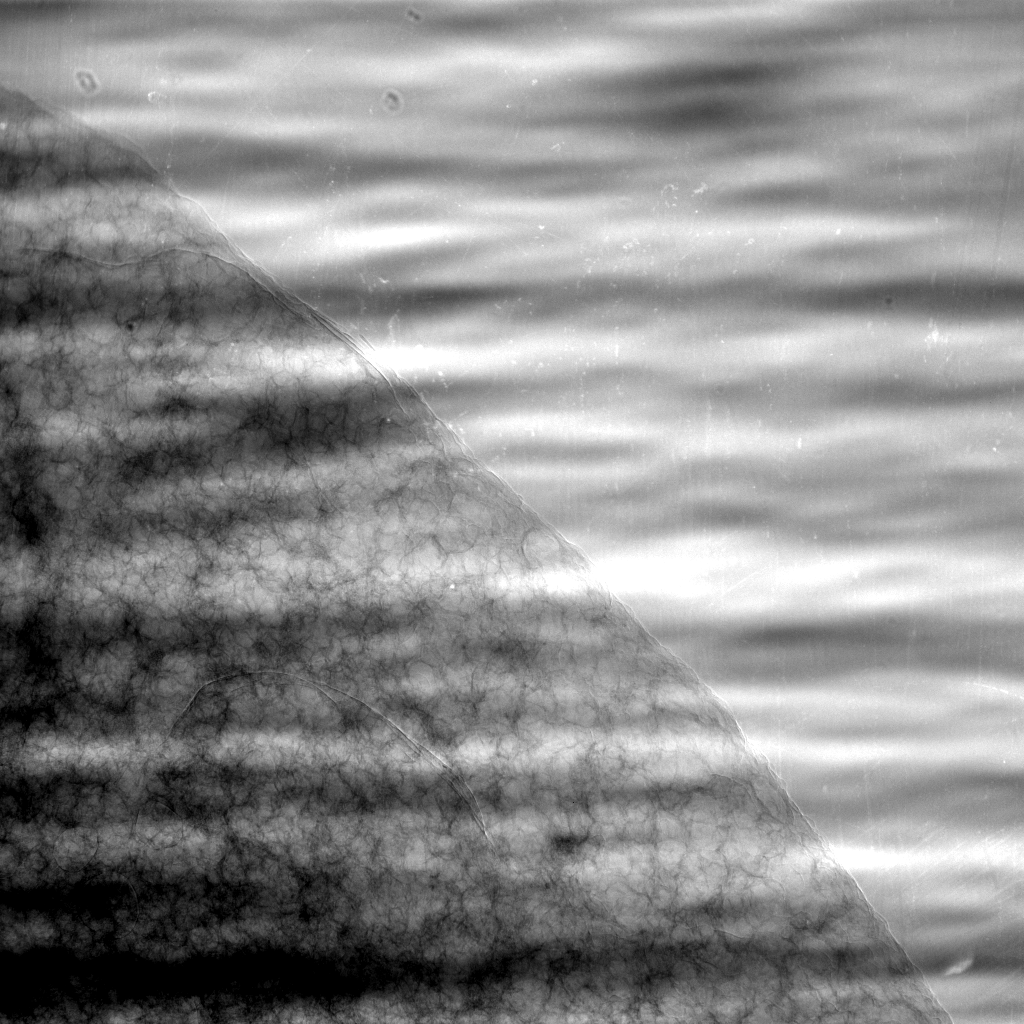
\includegraphics[width=\imagewidth]{R108C21Cb_s33358_normalize}};%
				\def\overlap{138}%
				\fill [yellow, nearly transparent] (1,1) rectangle (\overlap,1024);%
				\draw (1,1) rectangle (\overlap,1024);%
				\draw[|-|,color=white] (1,200) -- (1024,200) node [midway,above] {\SI{1.51552}{\milli\meter}};%
				\def\x{924}% 1024 - 100
				\def\y{922}% 1024 * .9 = 921.6
				\def\bar{338}% 100 px = 148 um
				\draw[|-|,color=white] (\x-\bar,\y) -- (\x,\y) node [midway,above] {\SI{500}{\micro\meter}};%
			\end{tikzpicture}%
			\label{fig:subscans}%
			}\\%
		\renewcommand{\imsize}{\linewidth}%
		\pgfmathsetlength{\imagewidth}{\imsize} % desired displayed width of image
		\pgfmathsetlength{\imagescale}{\imagewidth/2793}% pixel width of image
		\subfloat[Merged and corrected image from the three subscans shown in subfigure~\subref{fig:subscans}. Each merged projection has a size of 2793\(\times\)1024 pixels at a resolution of \SI{1.48}{\micro\meter\per pixel}. The width of the merged projections is slightly smaller than three times the width of the subscans due to the overlap needed to merge the projections (2793~px$=3\cdot3072$~px$-141$~px$-138$~px). Since the x-ray beam is extremely stable, the bands visible in the raw projections can be eliminated.]{%
			\begin{tikzpicture}[x=\imagescale,y=-\imagescale]%
				\node[anchor=north west,inner sep=0pt,outer sep=0pt] at (0,0)%
					{\includegraphics[width=\imagewidth]{R108C21Cb_mrg3333_normalize}};%
				\def\x{2693} % 2793-100
				\def\y{922} % 1024*.9 = 921.6
				\def\bar{338} % 100 px = 148 um
				\draw[|-|,color=white] (1,256) -- (2792,256) node [midway,above] {\SI{4.13364}{\milli\meter}};
				\draw[|-|,color=white] (\x-\bar,\y) -- (\x,\y) node [midway,above] {\SI{500}{\micro\meter}};
				\end{tikzpicture}%
			\label{fig:merge-proj}%
			}\\%
		\renewcommand{\imsize}{\linewidth}%
		\pgfmathsetlength{\imagewidth}{\imsize}% desired displayed width of image
		\pgfmathsetlength{\imagescale}{\imagewidth/2792}% pixel width of image (image has been resized from 2994*1123, so that scalebar is at the same height without calculating too much...)
		\subfloat[Cropped part of one slice of the tomographic dataset reconstructed from 5244 merged projections shown in subfigure~\subref{fig:merge-proj}. Due to the coherence of the x-ray beam the air-to-paraffin interface is visible around the sample.]{%
			\begin{tikzpicture}[x=\imagescale,y=-\imagescale]%
				% place image (integer coordinates refer to pixel centers):
				\node [anchor=north west,inner sep=0pt,outer sep=0pt] at (0,0)%
					{\includegraphics[width=\imagewidth]{R108C21Cb_mrg1024rec8bit}};% ``mogrify -shave 0x900 -normalize -format png R108C21Cb_mrg1024rec8bit.tif''
				\clip (0,0) rectangle (2792,992);				
				\def\x{2692} % 2708-100
				\def\y{893} % 992 * .9 = 892.8
				\def\bar{338} % 100 px = 148 um
				%%%% scalebar
					\draw[|-|,color=white] (\x-\bar,\y) -- (\x,\y) node [midway,above] {\SI{500}{\micro\meter}};
					\draw[|-|,color=white] (1,20) -- (2792,20) node [midway,below] {\SI{4.13216}{\milli\meter}};
				%%%% center
					\fill [color=red] (2792/2,992/2) circle (5);
				%%%% big circle
					\draw [dashed,color=red] (2792/2,992/2) circle (512);
					\def\angle{45}
					\draw [white,<->] (2792/2,992/2) +(\angle:0) --  node (bigto) {} +(\angle:512); 
					\node [white] (bigfrom) at (256,256){$\frac{1024}{2}$px};
					\draw [white,->,densely dotted] (bigfrom) to [bend left=45] (bigto);
				%%%% big circle
				%%%% 141px circle
				\draw [dashed,color=red] (2792/2,992/2) circle (512-141);
				\def\angle{45+90}
					\draw [white,<->] (2792/2,992/2) +(\angle:0) -- node (smallto) {} +(\angle:512-141);
					\node [white] (smallfrom) at (256,384) {$\frac{1024}{2}-141$px};
					\draw [white,->,densely dotted] (smallfrom) to [bend left=45] (smallto);
				%%%% 141px circle					
%				%%%% 138px circle
%				\draw [dashed,color=red] (2792/2,992/2) circle (512-138);
%				\def\angle{45+90+90}
%					\draw [white,<->] (2792/2,992/2) +(\angle:0) -- node (vsmallto) {} +(\angle:512-138);
%					\node [white] (vsmallfrom) at (2972-768,992-512) {$\frac{1024}{2}-138$px};
%					\draw [white,->,densely dotted] (vsmallfrom) to [bend right=45] (vsmallto);
%				%%%% 138px circle
				%%%% inset
%				\newcommand{\size}{.2\imagewidth}%
%				\clip (256,256) rectangle (512,512);
%				\node[anchor=north west,inner sep=0pt,outer sep=0pt] at (0,0)
%					{\includegraphics[width=\size]{R108C21Cb_mrg1024rec8bit}};
%					\draw[white] (0,0) rectangle (\size,-\size);
				%%%% inset
				\end{tikzpicture}%
			\label{fig:merge-rec}%
			}%
%%%%%%%%%%%%%%%%%%%%%%%%%%%%%	
%	\caption{caption}
%\end{figure}
%\end{document}
		\caption{Wide field scan of a rat lung sample obtained from a Sprague-Dawley rat 21 days after birth, showing the distal-medial edge of the right lower lung lobe. The sample has been scanned at \SI{12.6}{\kilo\electronvolt}, the protocol details conform to protocol ``B'', described in table~\ref{tab:protocols}.}%
		\label{fig:wide field scan results}%
	\end{figure*}
\fi

\subsection{Increasing the field of view}
The field of view of classic tomographic scans at TOMCAT made it possible to visualize partial acini inside a three-dimensional dataset. Increasing the available field of view three times allows us to obtain three dimensional reconstructions of full acini inside the sample, we are not limited by the field of view, only by the available sample size. Figure~\ref{fig:s2-wfs} shows reconstructions for a conventional (fig.~\ref{fig:s2-wfs}a) and for a wide field scan (fig.~\ref{fig:s2-wfs}b). The increased field of view allows the visualization of third acinus (yellow) which is not visible inside the field of view of a conventional scan. In addition, it is also visible that both the red and green segment for the conventional scan are extend out of the field of view of the conventional scan, we need to record a wide field scan to visualize both these segments in three dimensions, as can be observed in figure~\ref{fig:s2-wfs}b). The red and yellow segment visualized for the wide field scan are still only partial acini, but their size is only limited by the dimensions of the lung sample, not by the imaging method.

\ifiucr
	%\onecolumn
	\begin{figure}%
		\centering%
		\caption{Three dimensional visualization of the distal-medial tip of the right lower lung lobe of a Sprague Dawley rat. The gray structure in the background shows a semitransparent view of the sample with segmented airways. The foreground shows isosurfaces of terminal airways that have been extracted using a threshold interval based region growing algorithm. a): Conventional scan; the extracted acini (green and red segments) are only partially visible inside the total sample volume. b): Wide field scan; the green and red segment show multiple full acini inside the dataset, the yellow segment contains on acinus only partially visible inside the total sample volume. The segmentation is only limited by the sample size and not by the field of view of the tomographic scan.}%
		\label{fig:s2-wfs}%
		\def\x{250}%
		\def\y{575}%
		\renewcommand{\imsize}{\linewidth}%
		\pgfmathsetlength{\imagewidth}{\imsize}%
		\pgfmathsetlength{\imagescale}{\imagewidth/1202}%
		\begin{tikzpicture}[x=\imagescale,y=-\imagescale]%
			\node[anchor=north west,inner sep=0pt,outer sep=0pt] at (0,0)%
				{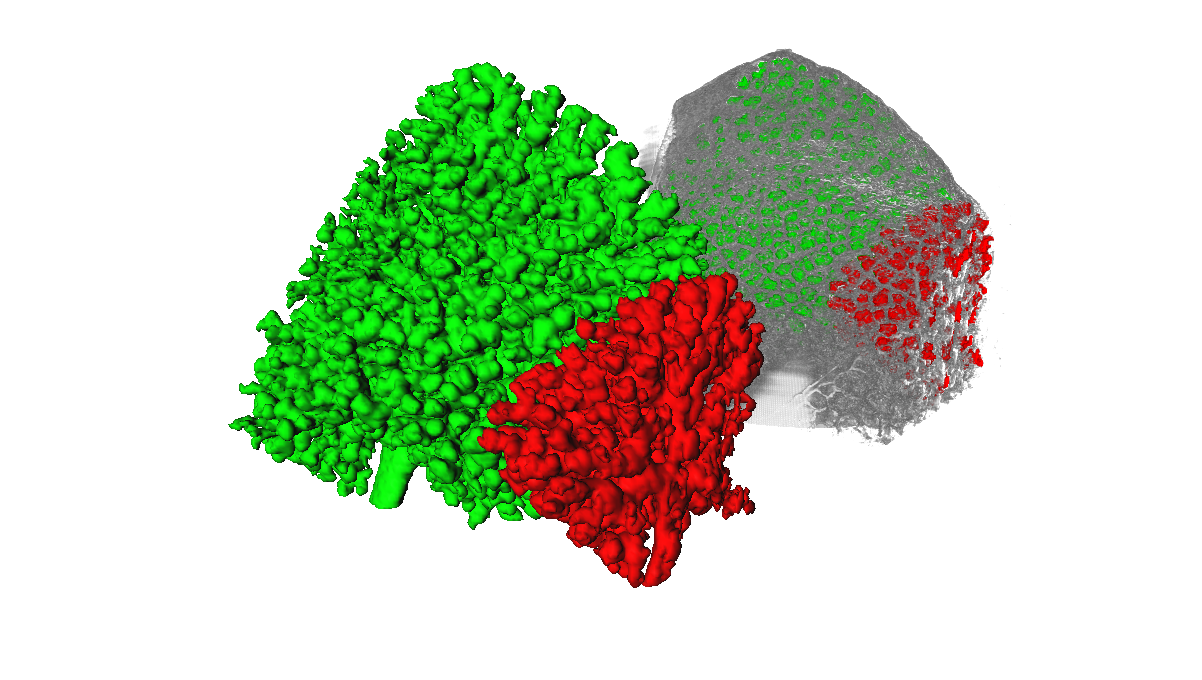
\includegraphics[width=\imagewidth]{img/widefieldscanning/R108C04C-overview-s2}};%
			% 510px = 1.5155mm > 100px = 297um > 168px = 500um
			\draw[|-|,thick] (244,367) -- (718,554) node [sloped,midway,above] {\SI{1.5155}{\milli\meter}};%
			\draw[|-|,thick] (\x,\y) -- (\x+168,\y) node [midway,above] {\SI{500}{\micro\meter}};%
		\end{tikzpicture}\\%
		a) Conventional scan\\%
		\renewcommand{\imsize}{\linewidth}%
		\pgfmathsetlength{\imagewidth}{\imsize}%
		\pgfmathsetlength{\imagescale}{\imagewidth/1202}%
		\def\x{150}%
		\def\y{575}%
		\begin{tikzpicture}[x=\imagescale,y=-\imagescale]%
			\node[anchor=north west,inner sep=0pt,outer sep=0pt] at (0,0)%
				{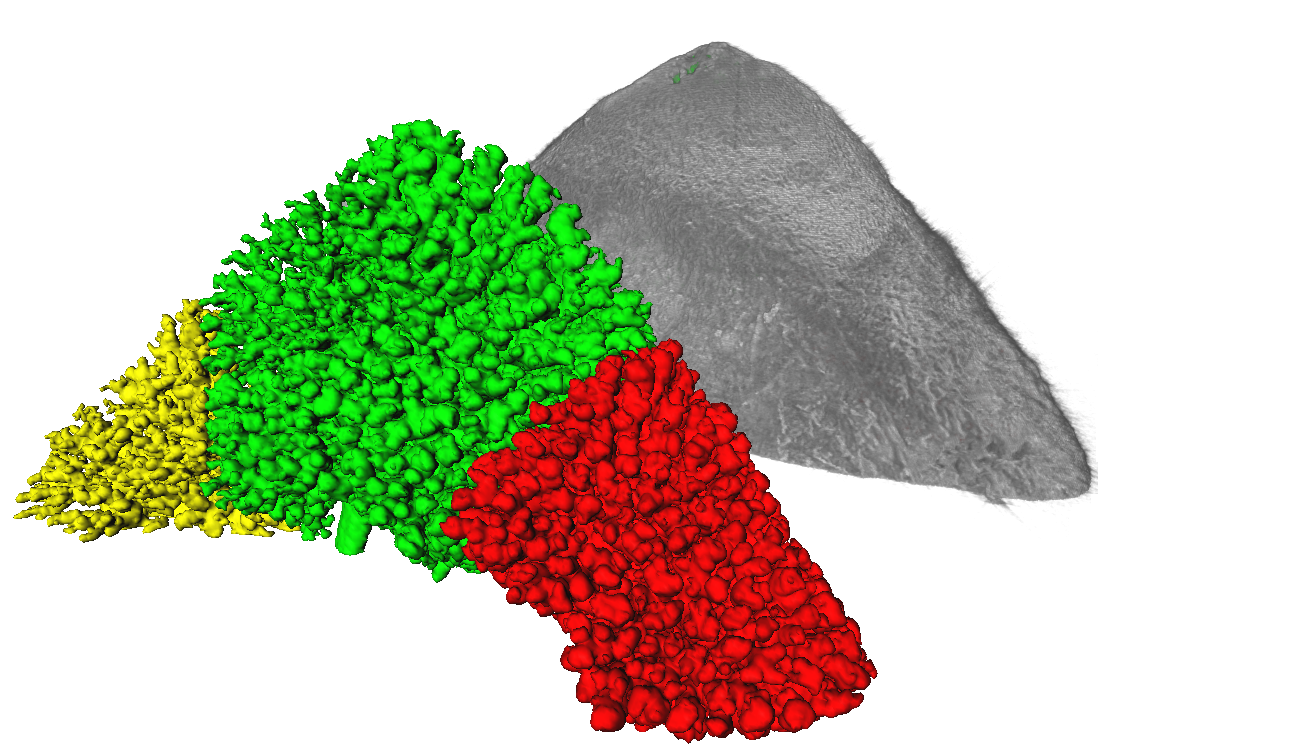
\includegraphics[width=\imagewidth]{img/widefieldscanning/R108C04C-overview-merge}};%
			% 906px = 4.0641mm > 100px = 449um > 111px = 500um
			\draw[|-|,thick] (39,454) -- (923,653) node [sloped,midway,above] {\SI{4.0641}{\milli\meter}};%
			\draw[|-|,thick] (\x,\y) -- (\x+222,\y) node [midway,above] {\SI{1}{\milli\meter}};%
		\end{tikzpicture}\\%
		b) Scan with increased field of view\\%
	\end{figure}%
	%\twocolumn
\else
	\begin{figure}[htp]%
	\renewcommand{\imsize}{\linewidth}%
	\pgfmathsetlength{\imagewidth}{\imsize}% desired displayed width of image
	\pgfmathsetlength{\imagescale}{\imagewidth/1202}% pixel width of imagefile used below
		\centering%
		\def\x{250}%
		\def\y{575}%
		\subfloat[Conventional scan]{%
			\label{subfig:overview-s2}%
			\begin{tikzpicture}[x=\imagescale,y=-\imagescale]
				\node[anchor=north west,inner sep=0pt,outer sep=0pt] at (0,0)
					{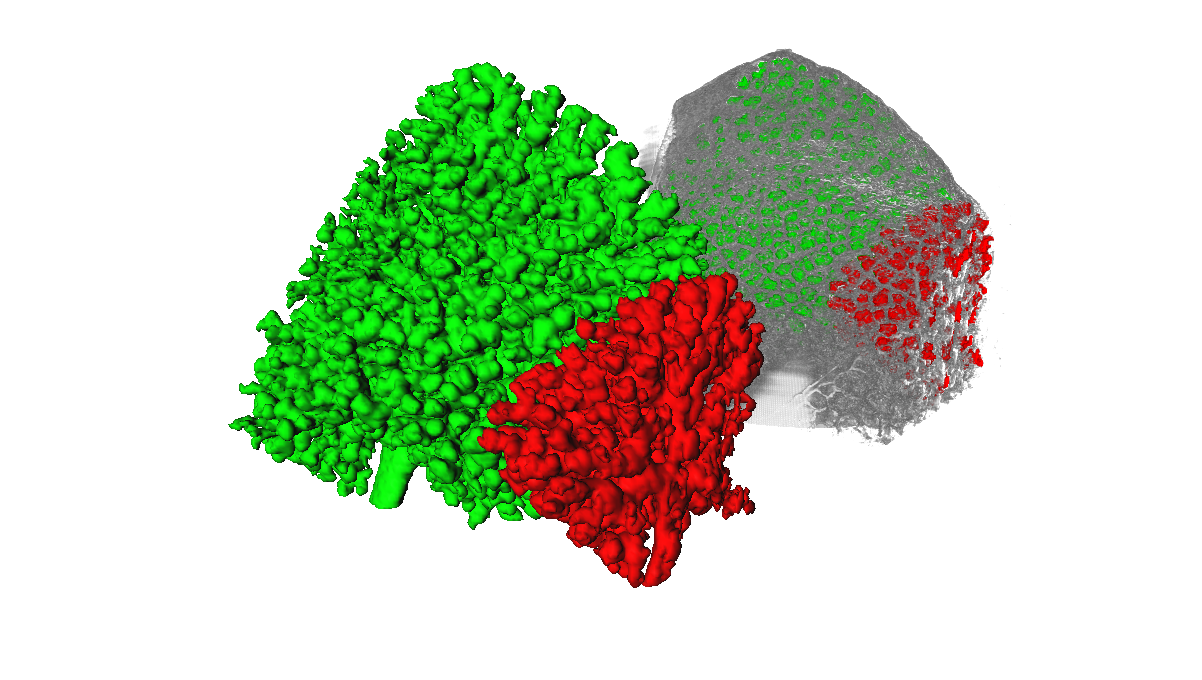
\includegraphics[width=\imagewidth]{img/widefieldscanning/R108C04C-overview-s2}};
				% 510px = 1.5155mm > 100px = 297um > 168px = 500um
				\draw[|-|,thick] (244,367) -- (718,554) node [sloped,midway,above] {\SI{1.5155}{\milli\meter}};
				\draw[|-|,thick] (\x,\y) -- (\x+168,\y) node [midway,above] {\SI{500}{\micro\meter}};
			\end{tikzpicture}%
		}\\%
		\def\x{150}%
		\def\y{575}%
		\subfloat[Scan with increased field of view]{%
			\label{subfig:overview-merge}%
			\begin{tikzpicture}[x=\imagescale,y=-\imagescale]
				\node[anchor=north west,inner sep=0pt,outer sep=0pt] at (0,0)
					{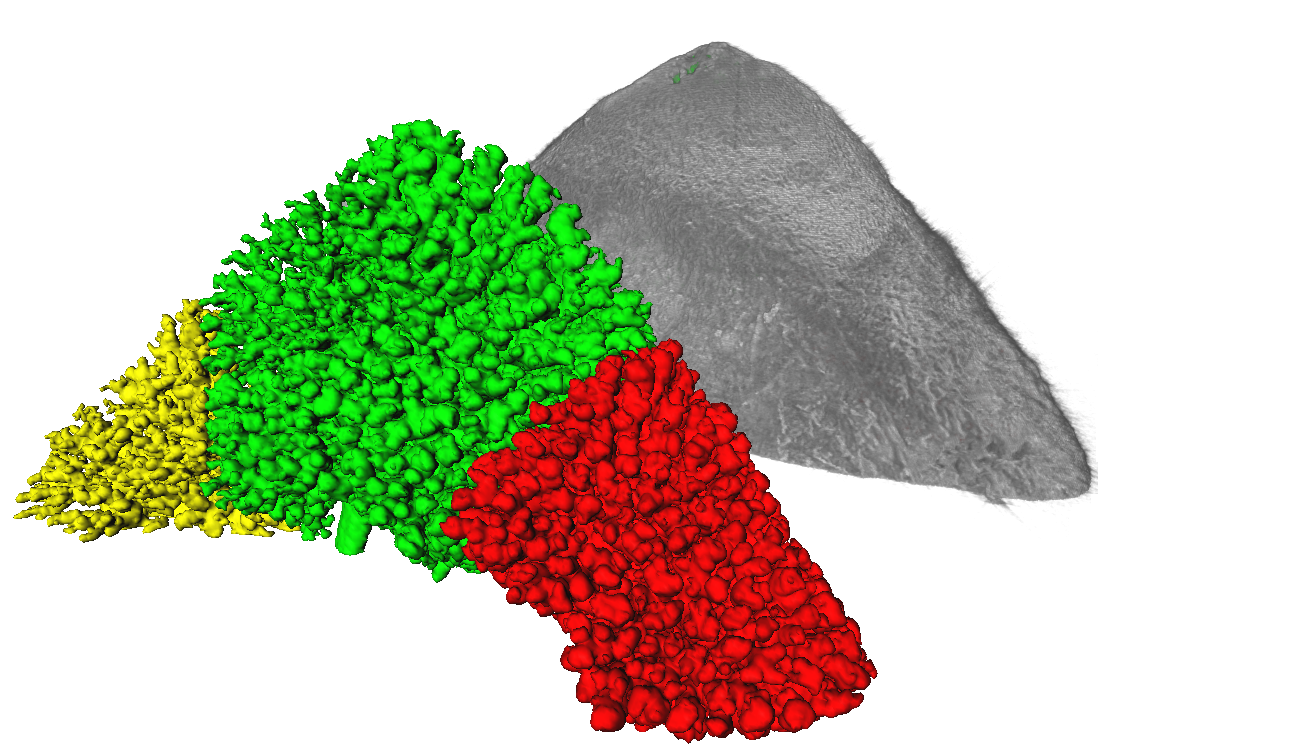
\includegraphics[width=\imagewidth]{img/widefieldscanning/R108C04C-overview-merge}};
				% 906px = 4.0641mm > 100px = 449um > 111px = 500um
				\draw[|-|,thick] (39,454) -- (923,653) node [sloped,midway,above] {\SI{4.0641}{\milli\meter}};
				\draw[|-|,thick] (\x,\y) -- (\x+222,\y) node [midway,above] {\SI{1}{\milli\meter}};
			\end{tikzpicture}%
		}%
		\caption{Three dimensional visualization of the distal-medial tip of the right lower lung lobe of a Sprague Dawley rat. The gray structure in the background shows a semitransparent view of the sample with segmented airways. The foreground shows isosurfaces of terminal airways that have been extracted using a threshold interval based region growing algorithm. a): Conventional scan; the extracted acini (green and red segments) are only partially visible inside the total sample volume. b): Wide field scan; the green and red segment show multiple full acini inside the dataset, the yellow segment contains on acinus only partially visible inside the total sample volume. The segmentation is only limited by the sample size and not by the field of view of the tomographic scan.}%
		\label{fig:s2-wfs}%
	\end{figure}
\fi

\subsection{Quality guided protocols}%
Table~\ref{tab:protocols} provides the numbers for the 19 different protocols that have been scanned for this manuscript. Protocol A would correspond to the scanning configuration shown in figure~\ref{subfig:goldstandard3}, which would require nine independent small scans, nine independent reconstructions and stitching of the resulting small datasets into one big dataset. As shown above, we can equally satisfy the sampling theorem when enough projections are acquired for a simulated detector size that is three times the real detector size of 1024 pixels, so protocol A was omitted for this study. Including an overlap of 100 pixels between the central and the ring scan, we need to acquire $P_{B}=15419$ projections for the gold-standard protocol B ($P_{B}=3(3072+200)\frac{\pi}{2}$). The protocols C--T have been linearly scaled down with a decreasing percentage of acquired total projections of the gold standard.

\begin{table}
	\caption{Specification of different protocols and time used compared to gold standard. Protocol A corresponds to the Gold Standard, and would have been needed to cover the same field of view with 9 independent scans with a detector width of 1024 pixels (plus an overlap of 100 pixels), resulting in a number of projections $P_{A}=9*(1024+100)\ifhtml \pi/2 \else \frac{\pi}{2} \fi= 15890$. Protocol B corresponds to the protocol shown in figure~\ref{fig:Setup3SubScans}c), resulting in a total number of projections of $P_{B} = 3(3072+200)\ifhtml \pi/2 \else \frac{\pi}{2} \fi= 15419$.}%
	\label{tab:protocols}%
	\centering%
	\begin{tabular}{rccccc}%
		Protocol & $s_{1}$ & $s_{2}$ & $s_{3}$ & $\sum s_{1}:s_{3}$ & Time [\%]\\
		\hline%
		A &      &      &      & 15890 & 100.00\\%
		B & 5244 & 5244 & 5244 & 15732 &  99.01\\%
		C & 5244 & 2622 & 5244 & 13110 &  82.50\\%
		D & 4370 & 4370 & 4370 & 13110 &  82.50\\%
		E & 4370 & 2185 & 4370 & 10925 &  68.75\\%
		F & 3934 & 3934 & 3934 & 11802 &  74.27\\%
		G & 3934 & 1967 & 3934 &  9835 &  61.89\\%
		H & 3496 & 3496 & 3496 & 10488 &  66.00\\%
		I & 3496 & 1748 & 3496 &  8740 &  55.00\\%
		J & 3060 & 3060 & 3060 &  9180 &  57.77\\%
		K & 3060 & 1530 & 3060 &  7650 &  48.14\\%
		L & 2622 & 2622 & 2622 &  7866 &  49.50\\%
		M & 2622 & 1311 & 2622 &  6555 &  41.25\\%
		N & 2186 & 2186 & 2186 &  6558 &  41.27\\%
		O & 2185 & 1093 & 2185 &  5463 &  34.38\\%
		P & 1748 & 1748 & 1748 &  5244 &  33.00\\%
		Q & 1748 &  874 & 1748 &  4370 &  27.50\\%
		R & 1312 & 1312 & 1312 &  3936 &  24.77\\%
		S &  874 &  874 &  874 &  2622 &  16.50\\%
		T &  874 &  437 &  874 &  2185 &  13.75\\%
	\end{tabular}%
\end{table}

We were able to reduce the total acquisition time by \SI{86.25}{\percent} compared to the gold standard, as can be seen in table~\ref{tab:protocols}. All 19 protocols have been scanned, reconstructed and visualized three-dimensionally to assess the artifacts which arise through the reduction of the amount of projections. Albeit the maximally assessed reduction in scanning time by \SI{86.25}{\percent} does introduce visible artifacts in the three-dimensional reconstruction (as shown in figure~\ref{fig:BvsT}), an automated segmentation of the airways is still possible.

Differences between the protocols have been calculated using the difference image of binarized slices, segmented according to%
\ifhtml
	~\citet{Otsu1979}
\else
	~\citeasnoun{Otsu1979}
\fi%
. The binarization of the images suppresses small variations in the gray values of the reconstructed slices and enables us to only take into account the pixels that differ between the 19 different protocols. The difference value ($E_{norm}$) plotted in figure~\ref{fig:NormalizedErrorPlot} has been calculated for each protocol $i=$1--19 according to equations~\ref{eq:errorcalculation-a}--\ref{eq:errorcalculation-c}. Using a thresholded slice $i$ of each protocol $Prot$ ($Slice_{Prot_{i}}$) and the corresponding slice $i$ of the gold standard protocol $B$ ($Slice_{B_{i}}$) we calculated the absolute difference image ($D_{Prot_{i}}$) of these two slices $i$. The sum of all pixels of this difference image yields a value ($E_{Prot_{norm_{i}}}$) for each slice $i$ of each Protocol $Prot$, which assesses the difference of the examined slice with the corresponding slice of the gold standard protocol. 

\begin{eqnarray}%
	D_{Prot_{i}} &=& |Slice_{B_{i}}-Slice_{Prot_{i}}|\label{eq:errorcalculation-a}\\%
	E_{Prot_{norm_{i}}} &=& \sum_{x}\sum_{y} D_{Prot_{i}}\label{eq:errorcalculation-b}\\%
    E_{Prot_{norm}} &=& \overline{E_{Prot_{norm_{i}}}}\label{eq:errorcalculation-c}%
\end{eqnarray}%

This combined difference value ($E_{Prot_{norm_{i}}}$) has been calculated for 205 regularly spaced slices ($i=1:5:1024$) of the full dataset. The mean ($\overline{E_{Prot_{norm_{i}}}}$) difference value for all slices has been normalized to the scanned quality-steps from 20--\SI{100}{\percent} (as stated in table~\ref{tab:protocols}) and plotted as max$(E_{norm}-E_{Prot_{norm}})$ with its standard deviation ($\sigma(E_{Prot_{norm_{i}}})$), as can be observed in figure~\ref{fig:NormalizedErrorPlot}. The normalization and inversion has been done to make the plotted values directly comparable with each other.

The calculated quality of the reconstructions from the different protocols decreases with decreasing amount of total obtained projections, as predicted. Figure~\ref{fig:NormalizedErrorPlot} shows a plot of the calculated error of the different protocols compared to a gold standard protocol (blue diamonds), those are experimental results not derived using simulations with a phantom, but real data obtained from actual scans of lung tissue. Overlaid on this plot are the data obtained from simulations (red dots). Both the plots for the simulation and the normalized difference value are not perfectly in agreement, but show the same trend. The simulation shows an exponential decrease in quality, while the calculated, normalized error show a more linear decrease in quality from protocol B towards protocol T.

\ifiucr
	\begin{figure}%
		\centering%
		\caption{Plot of normalized difference Value ($E_{norm}$, blue diamonds) for the 19 scanned protocols overlaid over Quality-plot (red dots) obtained from the simulation. The normalized Error has been calculated using the difference image of each protocol $i$ with protocol B. The error bars for each protocol show the standard deviation of the error which was calculated for 205 of the 1024 slices for each protocol. Note that the scale of the error been normalized to 20--\SI{100}{\percent}, so that both the quality from the simulation and the error are directly comparable. The abscissa shows the scanning time in percentage of time used for the gold standard scan. The protocols would be shown are in decreasing order from T--B for increasing percentage.}%
		%\documentclass{article}
%\usepackage{tikz,pgfplots}
%\usepackage[pdftex,active,tightpage]{preview}
%\begin{document}
%\begin{preview}
%%%%%%%%%%%%%%%%%%%%%%%%%%%%%%
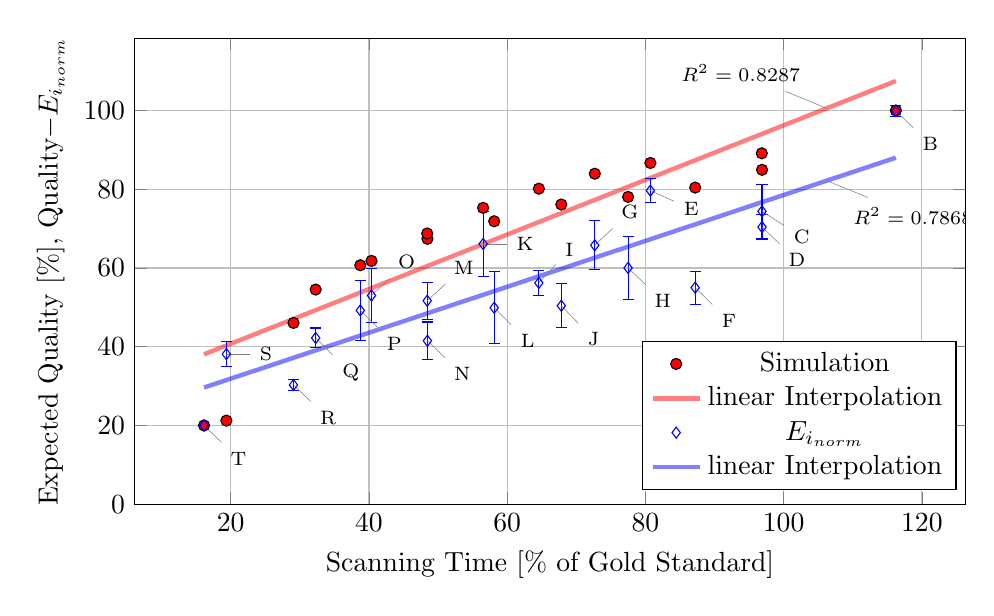
\begin{tikzpicture}

\pgfplotsset{every axis legend/.append style={at={(0.8,0.08)},anchor=base}}

\begin{axis}[%
	xmajorgrids,
  ymajorgrids,
	width=\linewidth,
	height=0.618\linewidth,
	%scale only axis,
	%xmin=0,%xmax=129,
	ymin=0,%ymax=125,
  xlabel={Scanning Time [\%\ of Gold Standard]},%
	ylabel={Expected Quality [\%], Quality$-E_{i_{norm}}$}%
	]

% Protocols
\addplot [ fill=red, only marks, mark = *]
	coordinates{
		(16.14,20)
		(19.37,21.2284)
		(29.08,46.0522)
		(32.29,54.5201)
		(38.75,60.7072)
		(40.37,61.8107)
		(48.46,67.4167)
		(48.43,68.7811)
		(58.12,71.8724)
		(56.52,75.28)
		(67.83,76.1345)
		(64.58,80.1592)
		(77.49,78.0612)
		(72.67,83.9645)
		(87.20,80.4284)
		(80.72,86.6889)
		(96.87,84.9458)
		(96.84,89.1421)
		(116.24,100)
};

\addplot [domain=16.14:116.24,color=red, semitransparent,ultra thick]
	{0.6936*x+26.891}; 

%% Line plot
%\addplot [smooth, solid, semitransparent]
	%coordinates{
		%(16.14,16.8548)
		%(19.37,25.9575)
		%(29.08,46.6567)
		%(32.29,51.7347)
		%(38.75,59.9714)
		%(40.37,61.6854) 
		%(48.46,68.6146)
		%(48.43,68.6305) 
		%(56.52,73.5452)
		%(58.12,74.3455)
		%(64.58,77.1605)
		%(67.83,78.3754)
		%(72.67,80.0091)
		%(77.49,81.5005)
		%(80.72,82.4599)
		%(87.20,84.3973)
		%(96.87,87.719)
%%		(96.87,87.719)
		%(116.24,99.8565)
%};

\addplot [ color=blue, only marks, mark=diamond ]
plot [ error bars/.cd, y dir=both, y explicit ]
    coordinates{
	( 16.14,20.0000) +- (0,0)      % T
	( 19.37,38.1358) +- (0,3.1135) % S
	( 29.08,30.2919) +- (0,1.3958) % R
	( 32.29,42.2255) +- (0,2.5278) % Q
	( 38.75,49.2247) +- (0,7.6789) % P
	( 40.37,53.0181) +- (0,6.8507) % O 
	( 48.46,41.5079) +- (0,4.7824) % N  
	( 48.43,51.6990) +- (0,4.7110) % M
	( 58.12,49.9058) +- (0,9.1839) % L
	( 56.52,66.1100) +- (0,8.1635) % K
	( 67.83,50.4137) +- (0,5.5671) % J
	( 64.58,56.2138) +- (0,3.2329) % I
	( 77.49,60.0243) +- (0,8.0805) % H
	( 72.67,65.7727) +- (0,6.2214) % G
	( 87.20,55.0069) +- (0,4.1882) % F
	( 80.72,79.6708) +- (0,3.0107) % E
	( 96.87,70.4018) +- (0,3.0863) % D
	( 96.87,74.3991) +- (0,6.8125) % C
	(116.24,99.8987) +- (0,1.3487) % B
};

\addplot [domain=16.14:116.24,color=blue, semitransparent,ultra thick]
	{0.5833*x+20.226}; 

\legend{%
	Simulation,%
	linear Interpolation,%
	$E_{i_{norm}}$,%
	linear Interpolation}

% \draw [<-] (axis cs:97.87,74.3991) -- (axis cs:99.87,74.3991) node [anchor=text] {\tiny C}; 
% \draw [<-] (axis cs:97.87,70.4018) -- (axis cs:99.87,70.4018) node [anchor=text] {\tiny D};
% \draw [<-] (axis cs:81.72,79.6708) -- (axis cs:82.72,79.6708) node [anchor=text] {\tiny E};
% \draw [<-] (axis cs:78.49,60.0243) -- (axis cs:79.49,60.0243) node [anchor=text] {\tiny H};
% \draw [<-] (axis cs:65.58,56.2138) -- (axis cs:66.58,56.2138) node [anchor=text] {\tiny I};
% \draw [<-] (axis cs:49.43,51.6990) -- (axis cs:51.43,51.6990) node [anchor=text] {\tiny M};
% \draw [<-] (axis cs:49.46,41.5079) -- (axis cs:51.46,41.5079) node [anchor=text] {\tiny N};

\tikzstyle{every pin}=[pin distance=2ex,font=\scriptsize]
\node[coordinate, pin=below right:{B}] at (axis cs:116.24,99.8987) {}; % B
\node[coordinate, pin=-22.5:{C}] at (axis cs:96.87,74.3991) {}; % C
\node[coordinate, pin=below right:{D}] at (axis cs:96.87,70.4018) {}; % D
\node[coordinate, pin=-5:{E}] at (axis cs:80.72,79.6708) {}; % E
\node[coordinate, pin=below right:{F}] at (axis cs:87.20,55.0069) {}; % F
\node[coordinate, pin=above right:{G}] at (axis cs:72.67,65.7727) {}; % G
\node[coordinate, pin=below right:{H}] at (axis cs:77.49,60.0243) {}; % H
\node[coordinate, pin=above right:{I}] at (axis cs:64.58,56.2138) {}; % I
\node[coordinate, pin=below right:{J}] at (axis cs:67.83,50.4137) {}; % J
\node[coordinate, pin=right:{K}] at (axis cs:56.52,66.1100) {}; % K
\node[coordinate, pin=below right:{L}] at (axis cs:58.12,49.9058) {}; % L
\node[coordinate, pin=above right:{M}] at (axis cs:48.43,51.6990) {}; % M
\node[coordinate, pin=below right:{N}] at (axis cs:48.46,41.5079) {}; % N  
\node[coordinate, pin=above right:{O}] at (axis cs:40.37,53.0181) {}; % O
\node[coordinate, pin=below right:{P}] at (axis cs:38.75,49.2247) {}; % P
\node[coordinate, pin=below right:{Q}] at (axis cs:32.29,42.2255) {}; % Q
\node[coordinate, pin=below right:{R}] at (axis cs:29.08,30.2919) {}; % R
\node[coordinate, pin=right:{S}] at (axis cs:19.37,38.1358) {}; % S
\node[coordinate, pin=below right:{T}] at (axis cs:16.14,20.0000) {}; % T

\node[coordinate, pin=above left:{$R^2=0.8287$}] at (axis cs:106.24,100.5791) {};
\node[coordinate, pin=below right:{$R^2=0.7868$}] at (axis cs:106.24, 82.1958) {};


\end{axis}

\end{tikzpicture}
%%%%%%%%%%%%%%%%%%%%%%%%%%%%%%
%\end{preview}
%\end{document}

%%%%%%%%%%%%%%%%%%%%%%%%%%%%%%
% plot erstellt mit MATLAB-File p:\\MATLAB\WideFieldScan/Paper/wfs_Compare2008c_ErrorPlot.m
% mit FromToTo = 1:5:1024
% sowie matlab2tikz
% Daten
%%%%%%%%%%Time =
%%%%%%%%%%  Columns 1 through 12
%%%%%%%%%%
%%%%%%%%%%   13.75   16.50   24.77   27.50   33   34.38   41.27   41.25   49.50   48.14   57.77   55
%%%%%%%%%%
%%%%%%%%%%  Columns 13 through 19
%%%%%%%%%%
%%%%%%%%%%   66   61.89   74.27   68.75   82.50   82.50   99.01
%MeanCumulativeError =
%
%  Columns 1 through 12
%
%   20.0000   38.1358   30.2919   42.2255   49.2247   53.0181   41.5079   51.6990   49.9058   66.1100   50.4137   56.2138
%
%  Columns 13 through 19
%
%   60.0243   65.7727   55.0069   79.6708   70.4018   74.3991   99.8987
%
%
%StandardDeviationofCumulativeError =
%
%  Columns 1 through 12
%
%         0    3.1135    1.3958    2.5278    7.6789    6.8507    4.7824    4.7110    9.1839    8.1635    5.5671    3.2329
%
%  Columns 13 through 19
%
%    8.0805    6.2214    4.1882    3.0107    3.0863    6.8125    1.3487
%%%%%%%%%%%%%%%%%%%%%%%%%%%%%%%
		\label{fig:NormalizedErrorPlot}%
	\end{figure}%
\else
	\begin{figure}[htp]
		\centering
		%\documentclass{article}
%\usepackage{tikz,pgfplots}
%\usepackage[pdftex,active,tightpage]{preview}
%\begin{document}
%\begin{preview}
%%%%%%%%%%%%%%%%%%%%%%%%%%%%%%
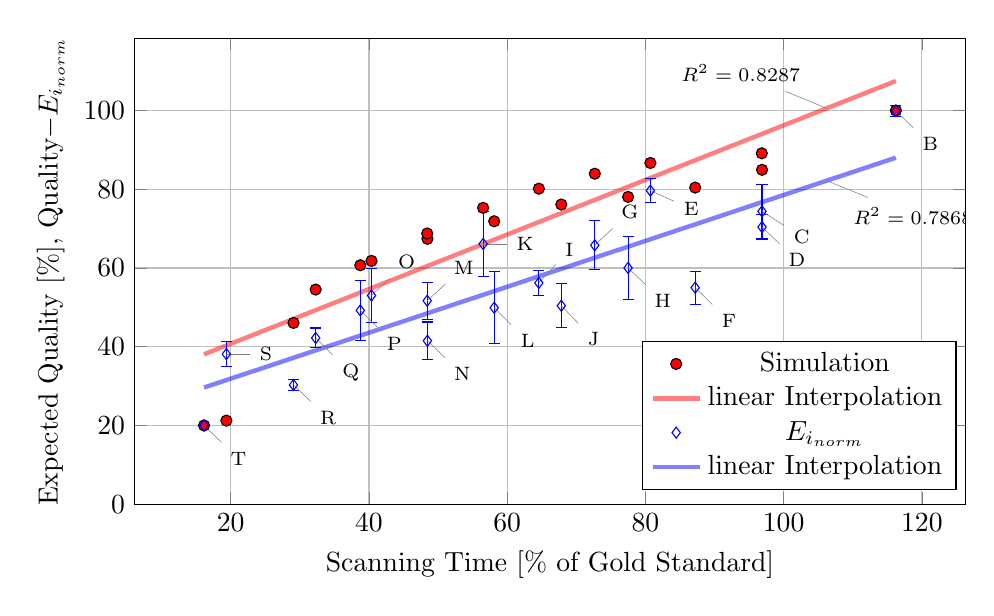
\begin{tikzpicture}

\pgfplotsset{every axis legend/.append style={at={(0.8,0.08)},anchor=base}}

\begin{axis}[%
	xmajorgrids,
  ymajorgrids,
	width=\linewidth,
	height=0.618\linewidth,
	%scale only axis,
	%xmin=0,%xmax=129,
	ymin=0,%ymax=125,
  xlabel={Scanning Time [\%\ of Gold Standard]},%
	ylabel={Expected Quality [\%], Quality$-E_{i_{norm}}$}%
	]

% Protocols
\addplot [ fill=red, only marks, mark = *]
	coordinates{
		(16.14,20)
		(19.37,21.2284)
		(29.08,46.0522)
		(32.29,54.5201)
		(38.75,60.7072)
		(40.37,61.8107)
		(48.46,67.4167)
		(48.43,68.7811)
		(58.12,71.8724)
		(56.52,75.28)
		(67.83,76.1345)
		(64.58,80.1592)
		(77.49,78.0612)
		(72.67,83.9645)
		(87.20,80.4284)
		(80.72,86.6889)
		(96.87,84.9458)
		(96.84,89.1421)
		(116.24,100)
};

\addplot [domain=16.14:116.24,color=red, semitransparent,ultra thick]
	{0.6936*x+26.891}; 

%% Line plot
%\addplot [smooth, solid, semitransparent]
	%coordinates{
		%(16.14,16.8548)
		%(19.37,25.9575)
		%(29.08,46.6567)
		%(32.29,51.7347)
		%(38.75,59.9714)
		%(40.37,61.6854) 
		%(48.46,68.6146)
		%(48.43,68.6305) 
		%(56.52,73.5452)
		%(58.12,74.3455)
		%(64.58,77.1605)
		%(67.83,78.3754)
		%(72.67,80.0091)
		%(77.49,81.5005)
		%(80.72,82.4599)
		%(87.20,84.3973)
		%(96.87,87.719)
%%		(96.87,87.719)
		%(116.24,99.8565)
%};

\addplot [ color=blue, only marks, mark=diamond ]
plot [ error bars/.cd, y dir=both, y explicit ]
    coordinates{
	( 16.14,20.0000) +- (0,0)      % T
	( 19.37,38.1358) +- (0,3.1135) % S
	( 29.08,30.2919) +- (0,1.3958) % R
	( 32.29,42.2255) +- (0,2.5278) % Q
	( 38.75,49.2247) +- (0,7.6789) % P
	( 40.37,53.0181) +- (0,6.8507) % O 
	( 48.46,41.5079) +- (0,4.7824) % N  
	( 48.43,51.6990) +- (0,4.7110) % M
	( 58.12,49.9058) +- (0,9.1839) % L
	( 56.52,66.1100) +- (0,8.1635) % K
	( 67.83,50.4137) +- (0,5.5671) % J
	( 64.58,56.2138) +- (0,3.2329) % I
	( 77.49,60.0243) +- (0,8.0805) % H
	( 72.67,65.7727) +- (0,6.2214) % G
	( 87.20,55.0069) +- (0,4.1882) % F
	( 80.72,79.6708) +- (0,3.0107) % E
	( 96.87,70.4018) +- (0,3.0863) % D
	( 96.87,74.3991) +- (0,6.8125) % C
	(116.24,99.8987) +- (0,1.3487) % B
};

\addplot [domain=16.14:116.24,color=blue, semitransparent,ultra thick]
	{0.5833*x+20.226}; 

\legend{%
	Simulation,%
	linear Interpolation,%
	$E_{i_{norm}}$,%
	linear Interpolation}

% \draw [<-] (axis cs:97.87,74.3991) -- (axis cs:99.87,74.3991) node [anchor=text] {\tiny C}; 
% \draw [<-] (axis cs:97.87,70.4018) -- (axis cs:99.87,70.4018) node [anchor=text] {\tiny D};
% \draw [<-] (axis cs:81.72,79.6708) -- (axis cs:82.72,79.6708) node [anchor=text] {\tiny E};
% \draw [<-] (axis cs:78.49,60.0243) -- (axis cs:79.49,60.0243) node [anchor=text] {\tiny H};
% \draw [<-] (axis cs:65.58,56.2138) -- (axis cs:66.58,56.2138) node [anchor=text] {\tiny I};
% \draw [<-] (axis cs:49.43,51.6990) -- (axis cs:51.43,51.6990) node [anchor=text] {\tiny M};
% \draw [<-] (axis cs:49.46,41.5079) -- (axis cs:51.46,41.5079) node [anchor=text] {\tiny N};

\tikzstyle{every pin}=[pin distance=2ex,font=\scriptsize]
\node[coordinate, pin=below right:{B}] at (axis cs:116.24,99.8987) {}; % B
\node[coordinate, pin=-22.5:{C}] at (axis cs:96.87,74.3991) {}; % C
\node[coordinate, pin=below right:{D}] at (axis cs:96.87,70.4018) {}; % D
\node[coordinate, pin=-5:{E}] at (axis cs:80.72,79.6708) {}; % E
\node[coordinate, pin=below right:{F}] at (axis cs:87.20,55.0069) {}; % F
\node[coordinate, pin=above right:{G}] at (axis cs:72.67,65.7727) {}; % G
\node[coordinate, pin=below right:{H}] at (axis cs:77.49,60.0243) {}; % H
\node[coordinate, pin=above right:{I}] at (axis cs:64.58,56.2138) {}; % I
\node[coordinate, pin=below right:{J}] at (axis cs:67.83,50.4137) {}; % J
\node[coordinate, pin=right:{K}] at (axis cs:56.52,66.1100) {}; % K
\node[coordinate, pin=below right:{L}] at (axis cs:58.12,49.9058) {}; % L
\node[coordinate, pin=above right:{M}] at (axis cs:48.43,51.6990) {}; % M
\node[coordinate, pin=below right:{N}] at (axis cs:48.46,41.5079) {}; % N  
\node[coordinate, pin=above right:{O}] at (axis cs:40.37,53.0181) {}; % O
\node[coordinate, pin=below right:{P}] at (axis cs:38.75,49.2247) {}; % P
\node[coordinate, pin=below right:{Q}] at (axis cs:32.29,42.2255) {}; % Q
\node[coordinate, pin=below right:{R}] at (axis cs:29.08,30.2919) {}; % R
\node[coordinate, pin=right:{S}] at (axis cs:19.37,38.1358) {}; % S
\node[coordinate, pin=below right:{T}] at (axis cs:16.14,20.0000) {}; % T

\node[coordinate, pin=above left:{$R^2=0.8287$}] at (axis cs:106.24,100.5791) {};
\node[coordinate, pin=below right:{$R^2=0.7868$}] at (axis cs:106.24, 82.1958) {};


\end{axis}

\end{tikzpicture}
%%%%%%%%%%%%%%%%%%%%%%%%%%%%%%
%\end{preview}
%\end{document}

%%%%%%%%%%%%%%%%%%%%%%%%%%%%%%
% plot erstellt mit MATLAB-File p:\\MATLAB\WideFieldScan/Paper/wfs_Compare2008c_ErrorPlot.m
% mit FromToTo = 1:5:1024
% sowie matlab2tikz
% Daten
%%%%%%%%%%Time =
%%%%%%%%%%  Columns 1 through 12
%%%%%%%%%%
%%%%%%%%%%   13.75   16.50   24.77   27.50   33   34.38   41.27   41.25   49.50   48.14   57.77   55
%%%%%%%%%%
%%%%%%%%%%  Columns 13 through 19
%%%%%%%%%%
%%%%%%%%%%   66   61.89   74.27   68.75   82.50   82.50   99.01
%MeanCumulativeError =
%
%  Columns 1 through 12
%
%   20.0000   38.1358   30.2919   42.2255   49.2247   53.0181   41.5079   51.6990   49.9058   66.1100   50.4137   56.2138
%
%  Columns 13 through 19
%
%   60.0243   65.7727   55.0069   79.6708   70.4018   74.3991   99.8987
%
%
%StandardDeviationofCumulativeError =
%
%  Columns 1 through 12
%
%         0    3.1135    1.3958    2.5278    7.6789    6.8507    4.7824    4.7110    9.1839    8.1635    5.5671    3.2329
%
%  Columns 13 through 19
%
%    8.0805    6.2214    4.1882    3.0107    3.0863    6.8125    1.3487
%%%%%%%%%%%%%%%%%%%%%%%%%%%%%%
		\caption{Plot of normalized difference Value ($E_{norm}$, blue diamonds) for the 19 scanned protocols overlaid over Quality-plot (red dots) obtained from the simulation. The normalized Error has been calculated using the difference image of each protocol $i$ with protocol B. The error bars for each protocol show the standard deviation of the error which was calculated for 205 of the 1024 slices for each protocol. Note that the scale of the error been normalized to 20--\SI{100}{\percent}, so that both the quality from the simulation and the error are directly comparable. The abscissa shows the scanning time in percentage of time used for the gold standard scan. The protocols would be shown are in decreasing order from T--B for increasing percentage.}%
		\label{fig:NormalizedErrorPlot}
	\end{figure}
\fi

For protocols with the same total amount of projections, but different configurations of amount of projections for the central and the ring scan we observed a difference in reconstruction quality (compare the marked protocols C and D as well as protocols M and N in figure~\ref{fig:NormalizedErrorPlot}). This difference arises through the fact that the differing amount of subscans acquired for the central and the subscan add up to the same total amount of projections, but contribute differently to the quality of the reconstruction. From this finding it seems desirable to choose a protocol with equal amounts of subscans for each of the three independent subscans instead of a protocol with the same total amount of projections, but a decreased amount of projections for the central scan. Since a reduced amount of projections for the central scan decrease the reconstruction quality for the central parts of the sample, this explanation seems natural. In addition, the interpolation of missing projections could introduce artifacts in the reconstruction which are suppressed when simply stitching projections without interpolation.

\subsubsection{Three dimensional visualization of different protocols}%
\label{subsec:comparison}%
The 19 different protocols have been three dimensionally visualized and analyzed using MeVisLab (Version 1.6.1 (2008-09-21 Release), MeVis Medical Solutions AG, Bremen, Germany). Using a region growing algorithm~\cite{wiki:regiongrowing}, airway segments have been extracted from the tomographic dataset.  A seed point for the region growing algorithm has been manually defined inside the airway lumen to extract connected airway segments inside the tomographic datasets. The coordinates of the individual seed points for the extracted airway segments have been kept constant for protocol B--T, so that the extracted airway segments can be compared directly with each other. Exemplary airway segments extracted for protocol B and T are shown in figure~\ref{fig:BvsT}.

The protocols shown in figure~\ref{fig:BvsT} are the two extremes of the 19 obtained protocols  in terms of scanning time. Protocol B is the gold standard, obtained with in total 15732 projections recorded in 65 minutes. Protocol T has been obtained in just \SI{13.75}{\percent} of the scanning time, with in total 2185 projections recorded in 12 minutes (\SI{13.75}{\percent} of 65 minutes would be 9 minutes, the 3 minute difference arises through the movement of the sample which cannot be reduced with the recording of less projections). The tomographic dataset from protocol B has been reconstructed from 5244 merged projection images, the dataset from protocol T has been reconstructed using only 874 merged projections. Even if we scanned protocol T while violating the sampling theorem, both samples still appear to be nearly identical in the three dimensional visualization. Except for small differences at the most lateral parts of the sample (yellow segment) the segmented airways appear to identical, even if the scanning time of protocol T has been reduced to \SI{13.75}{\percent} of the scanning time of protocol B.

Only at higher magnifications the artifacts introduced through the great reduction in scanning time become apparent. The blue cube inside the green airway segments in figures~\ref{fig:BvsT}a) and \ref{fig:BvsT}b) are shown as isosurface visualizations of the lung tissue (which exactly corresponds to the negative of the extracted airway segment) in figures~\ref{fig:BvsT}c) and \ref{fig:BvsT}d).

Both regions of interest show a cube with a side length of \SI{190}{\micro\meter}. We observe that the isosurface of the ROI of protocol T shown in figure~\ref{subfig:DetailROIT} appears rougher than the isosurface of protocol B shown in figure~\ref{subfig:DetailROIB}. This roughness is introduced through the wave-like artifacts visible in the original slice of the dataset of protocol T\todo{since figure 11 was nicked, we don't show this slice anymore\ldots} (not shown) which arise through the breaching of the sampling theorem, since we have only acquired 874 projections for the outer scan (2185 projections in total for protocol T) instead of the 5139 projections ($(3072+200)\frac{\pi}{2}$) that would be necessary to satisfy the sampling theorem. But even with this strong undersampling a segmentation, three dimensional reconstruction and visualization of the sample is still possible. Thus, if the user desired to gain a quick overview over his sample, e.g.\ to quickly assess the integrity of multiple samples over a short time, such a time-saving protocol could be used.

\ifiucr%%% iucr %%%
	%\onecolumn%
	\begin{figure}%
		\centering%
		\caption{Comparison of three-dimensional visualizations of protocols B and T. Top: Three independent airway segments (green, red, yellow) have been extracted using a region growing algorithm. A cubical region of interest (ROI, blue) with a side length of 128 pixels (corresponding to \SI{190}{\micro\meter}) is marked inside the leftmost segment for both protocols. Bottom: Detailed view of isosurfaces of the lung tissue inside the ROIs shown above. Note the artifacts in the reconstructions for protocol T in subfigure d).}%
		\begin{tabular}{cc}%
			\renewcommand{\imsize}{.5\linewidth}%
			\pgfmathsetlength{\imagewidth}{\imsize}%
			\pgfmathsetlength{\imagescale}{\imagewidth/1397}%
			\def\x{100}%
			\def\y{150}%
			\begin{tikzpicture}[x=\imagescale,y=-\imagescale]%
				\node[anchor=north west,inner sep=0pt,outer sep=0pt] at (0,0)%
					{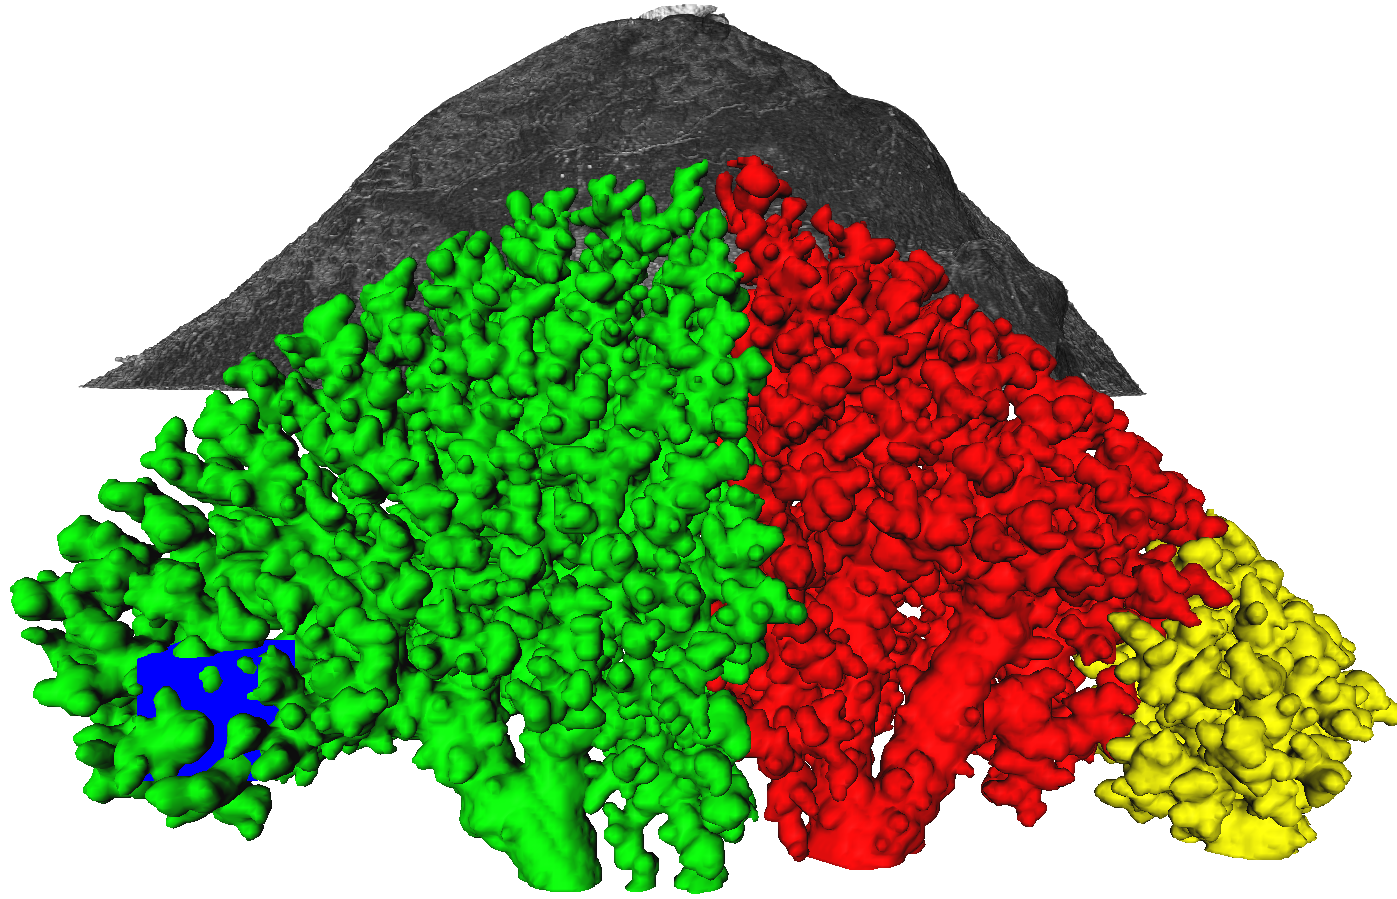
\includegraphics[width=\imagewidth]{img/comparisonBvsT/overview-b}};%
				% 1391px = 4.0138mm > 100px = 288um > 173px = 500um
				\draw[|-|,thick] (6,774) -- (1395,839) node [sloped,midway,above] {\SI{4.0138}{\milli\meter}};%
				\draw[|-|,thick] (\x,\y) -- (\x+173,\y) node [midway,above] {\SI{500}{\micro\meter}};%
			\end{tikzpicture}%
			\label{subfig:DetailOverviewB}%
		&%
			\renewcommand{\imsize}{.5\linewidth}%
			\pgfmathsetlength{\imagewidth}{\imsize}%
			\pgfmathsetlength{\imagescale}{\imagewidth/1397}%
			\def\x{100}%
			\def\y{150}%
			\begin{tikzpicture}[x=\imagescale,y=-\imagescale]%
				\node[anchor=north west,inner sep=0pt,outer sep=0pt] at (0,0)%
					{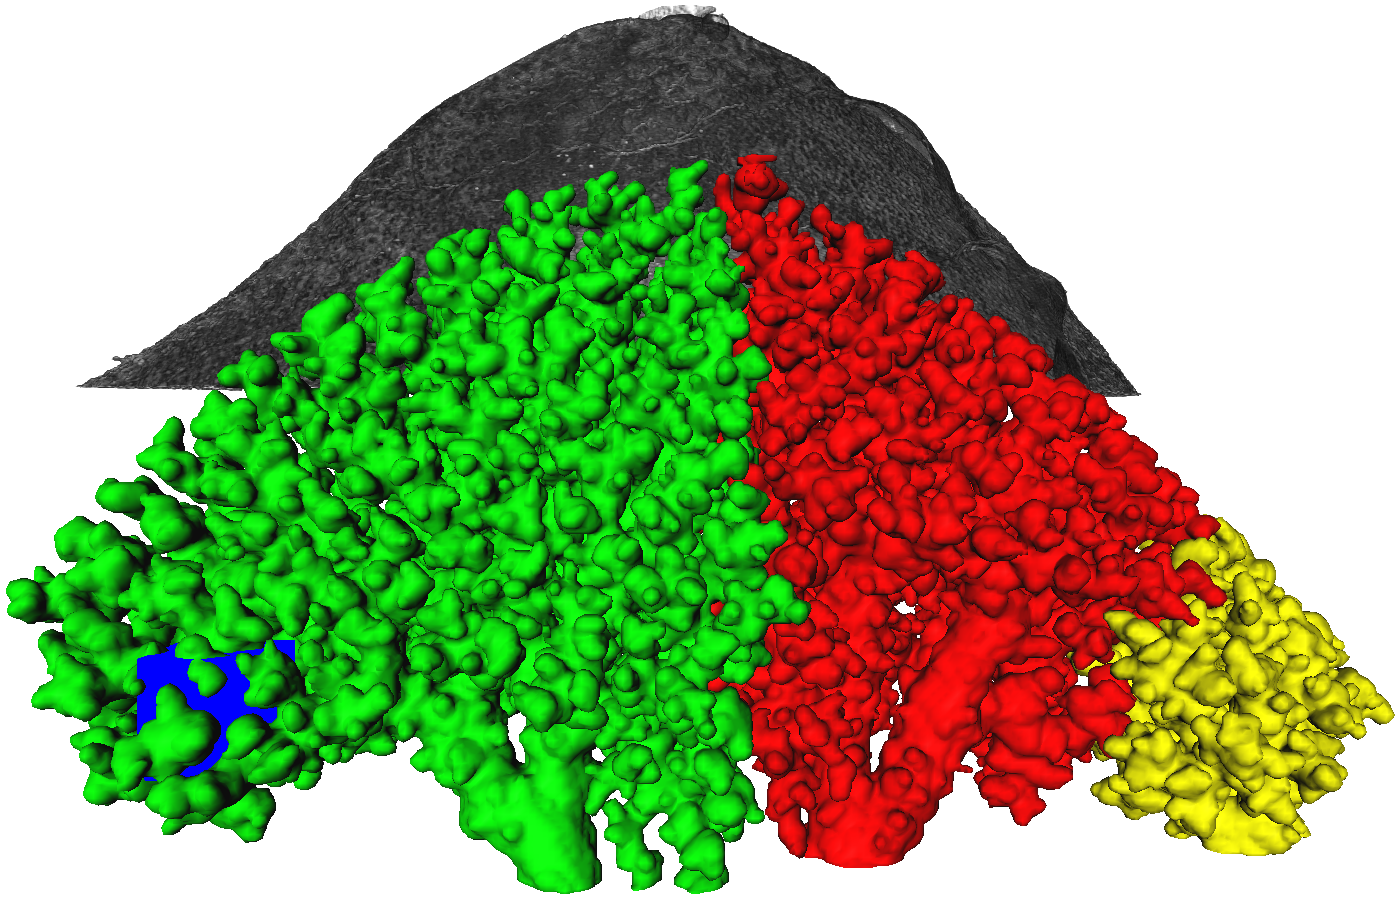
\includegraphics[width=\imagewidth]{img/comparisonBvsT/overview-t}};%
				% 1391px = 4.0138mm > 100px = 288um > 173px = 500um
				\draw[|-|,thick] (6,774) -- (1395,839) node [sloped,midway,above] {\SI{4.0138}{\milli\meter}};%
				\draw[|-|,thick] (\x,\y) -- (\x+173,\y) node [midway,above] {\SI{500}{\micro\meter}};%
			\end{tikzpicture}%
			\label{subfig:DetailOverviewT}%
		\\%
			a) Overview of protocol B%
		&%
			b) Overview of protocol T%
		\\%
			\renewcommand{\imsize}{.5\linewidth}%
			\pgfmathsetlength{\imagewidth}{\imsize}%
			\pgfmathsetlength{\imagescale}{\imagewidth/806}%
			\def\x{345}%
			\def\y{780}%
			\label{subfig:DetailROIB}%
			\begin{tikzpicture}[x=\imagescale,y=-\imagescale]%
				\node[anchor=north west,inner sep=0pt,outer sep=0pt] at (0,0)%
					{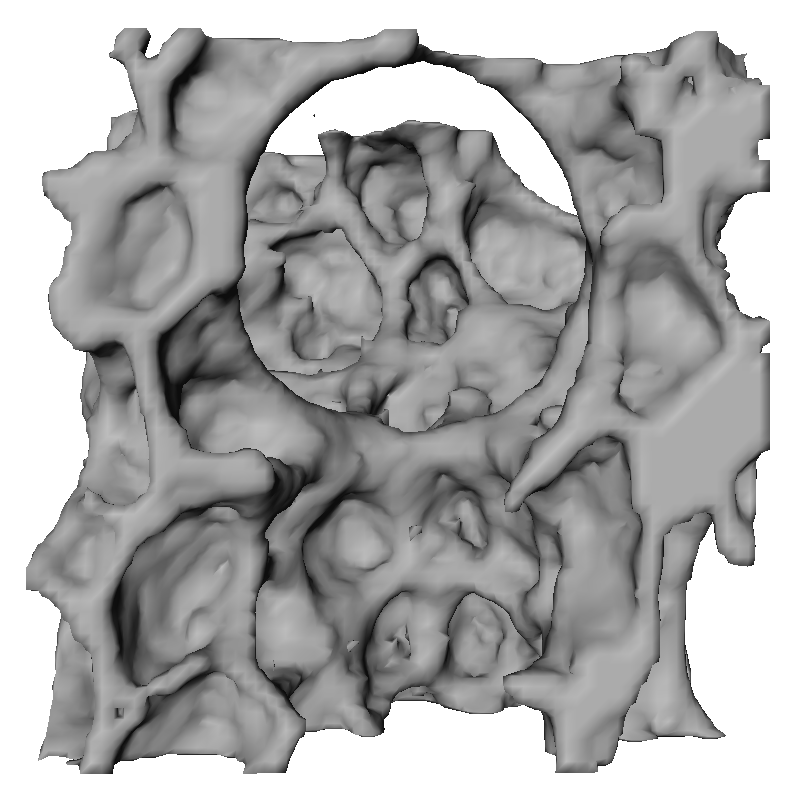
\includegraphics[width=\imagewidth]{img/comparisonBvsT/roi-b-nomedian}};%
				% 746px = 0.18944mm > 100px = 25um > 196.9px = 50um
				\draw[|-|,thick] (27,270) -- (773,272) node [sloped,midway,above] {\SI{189.44}{\micro\meter}};%
				\draw[|-|,thick] (\x,\y) -- (\x+196.9,\y) node [midway,above] {\SI{50}{\micro\meter}};%
			\end{tikzpicture}%
		&%
			\renewcommand{\imsize}{.5\linewidth}%
			\pgfmathsetlength{\imagewidth}{\imsize}%
			\pgfmathsetlength{\imagescale}{\imagewidth/806}%
			\def\x{345}%
			\def\y{780}%
			\label{subfig:DetailROIT}%
			\begin{tikzpicture}[x=\imagescale,y=-\imagescale]%
				\node[anchor=north west,inner sep=0pt,outer sep=0pt] at (0,0)%
					{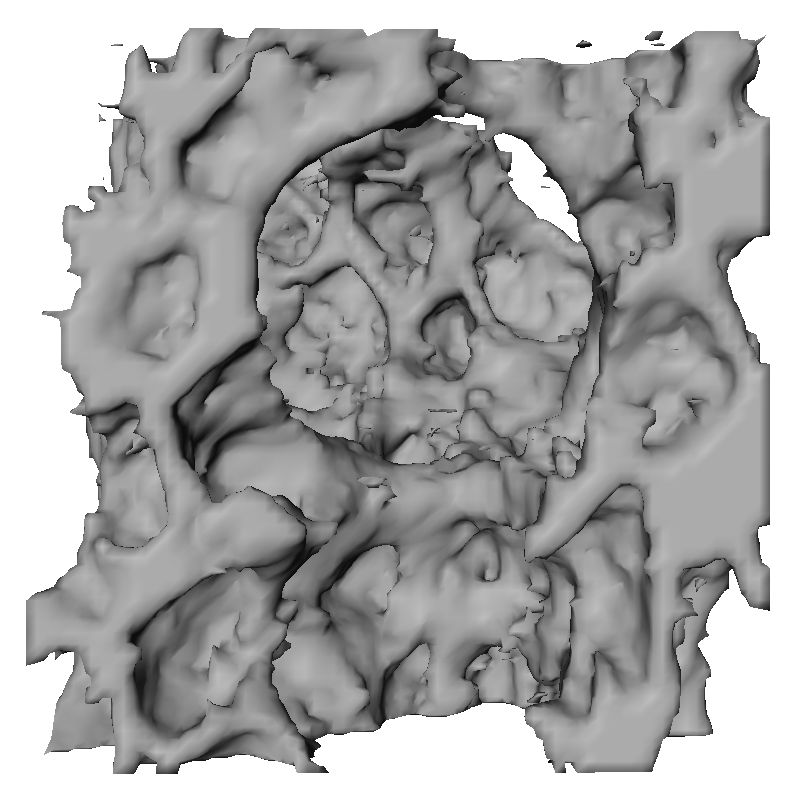
\includegraphics[width=\imagewidth]{img/comparisonBvsT/roi-t-nomedian}};%
				% 744px = 0.18944mm > 100px = 25um > 196.5px = 50um
				\draw[|-|,thick] (27,311) -- (771,311) node [sloped,midway,above] {\SI{189.44}{\micro\meter}};%
				\draw[|-|,thick] (\x,\y) -- (\x+196.5,\y) node [midway,above] {\SI{50}{\micro\meter}};%
			\end{tikzpicture}%
		\\%
			c) ROI inside green segment for protocol B%
		&%
			d) ROI inside green segment for protocol T%
		\\%
		\end{tabular}%
		\label{fig:BvsT}%
	\end{figure}%
\else
	\begin{figure*}[htp]
		\renewcommand{\imsize}{.5\linewidth}
		\centering
		\pgfmathsetlength{\imagewidth}{\imsize}          % desired displayed width of image
		\pgfmathsetlength{\imagescale}{\imagewidth/1397} % pixel width of imagefile used
		\def\x{100}
		\def\y{150}
		\subfloat[Overview of protocol B]{%
			\label{subfig:DetailOverviewB}%
			\begin{tikzpicture}[x=\imagescale,y=-\imagescale]
				\node[anchor=north west,inner sep=0pt,outer sep=0pt] at (0,0)
					{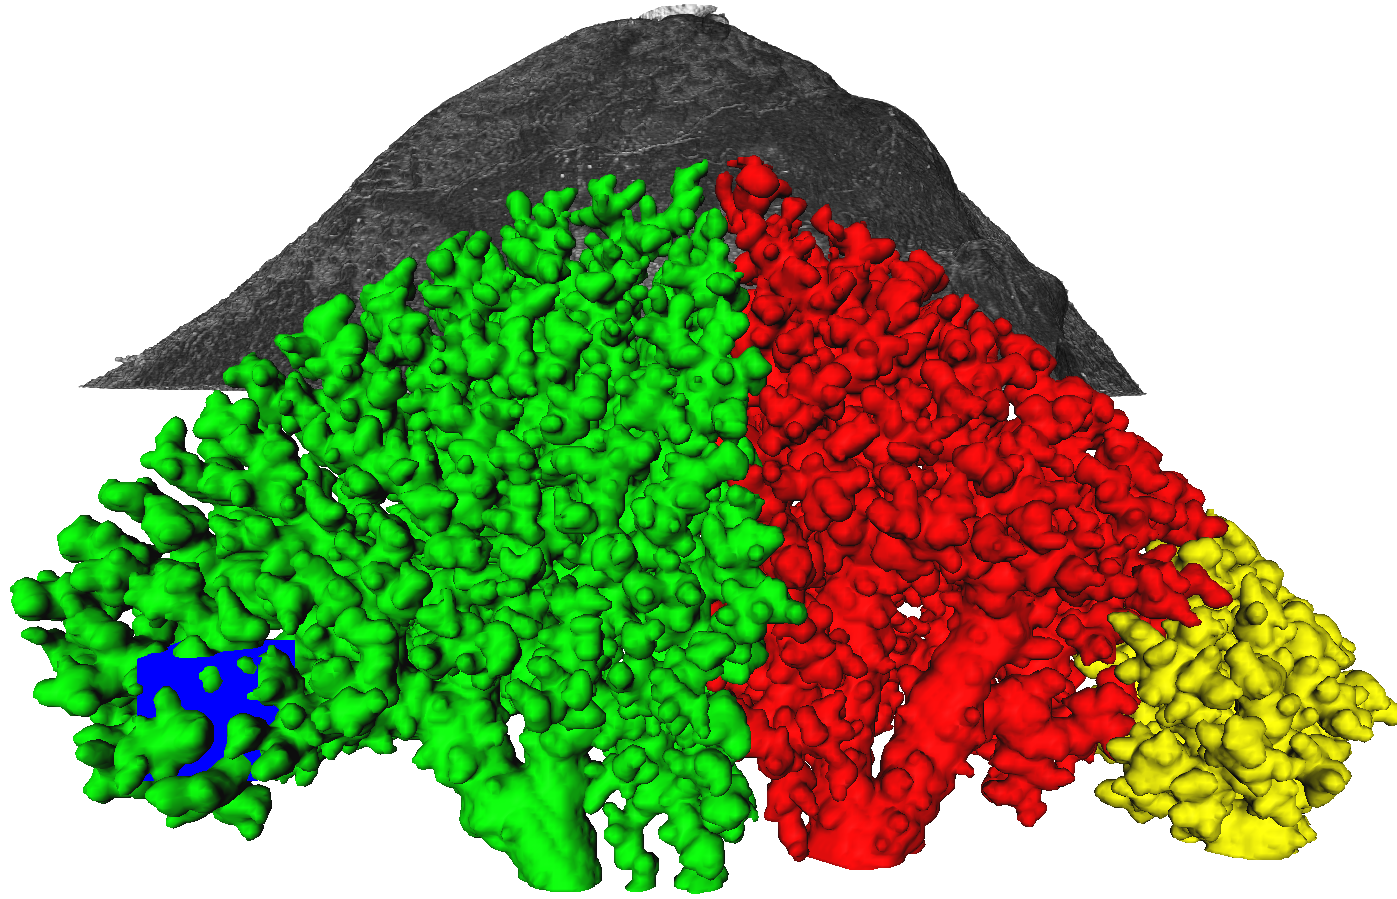
\includegraphics[width=\imagewidth]{img/comparisonBvsT/overview-b}};
				% 1391px = 4.0138mm > 100px = 288um > 173px = 500um
				\draw[|-|,thick] (6,774) -- (1395,839) node [sloped,midway,above] {\SI{4.0138}{\milli\meter}};
				\draw[|-|,thick] (\x,\y) -- (\x+173,\y) node [midway,above] {\SI{500}{\micro\meter}};
			\end{tikzpicture}%
			}%
		\subfloat[Overview of protocol T]{%
			\label{subfig:DetailOverviewT}%
			\begin{tikzpicture}[x=\imagescale,y=-\imagescale]
				\node[anchor=north west,inner sep=0pt,outer sep=0pt] at (0,0)
					{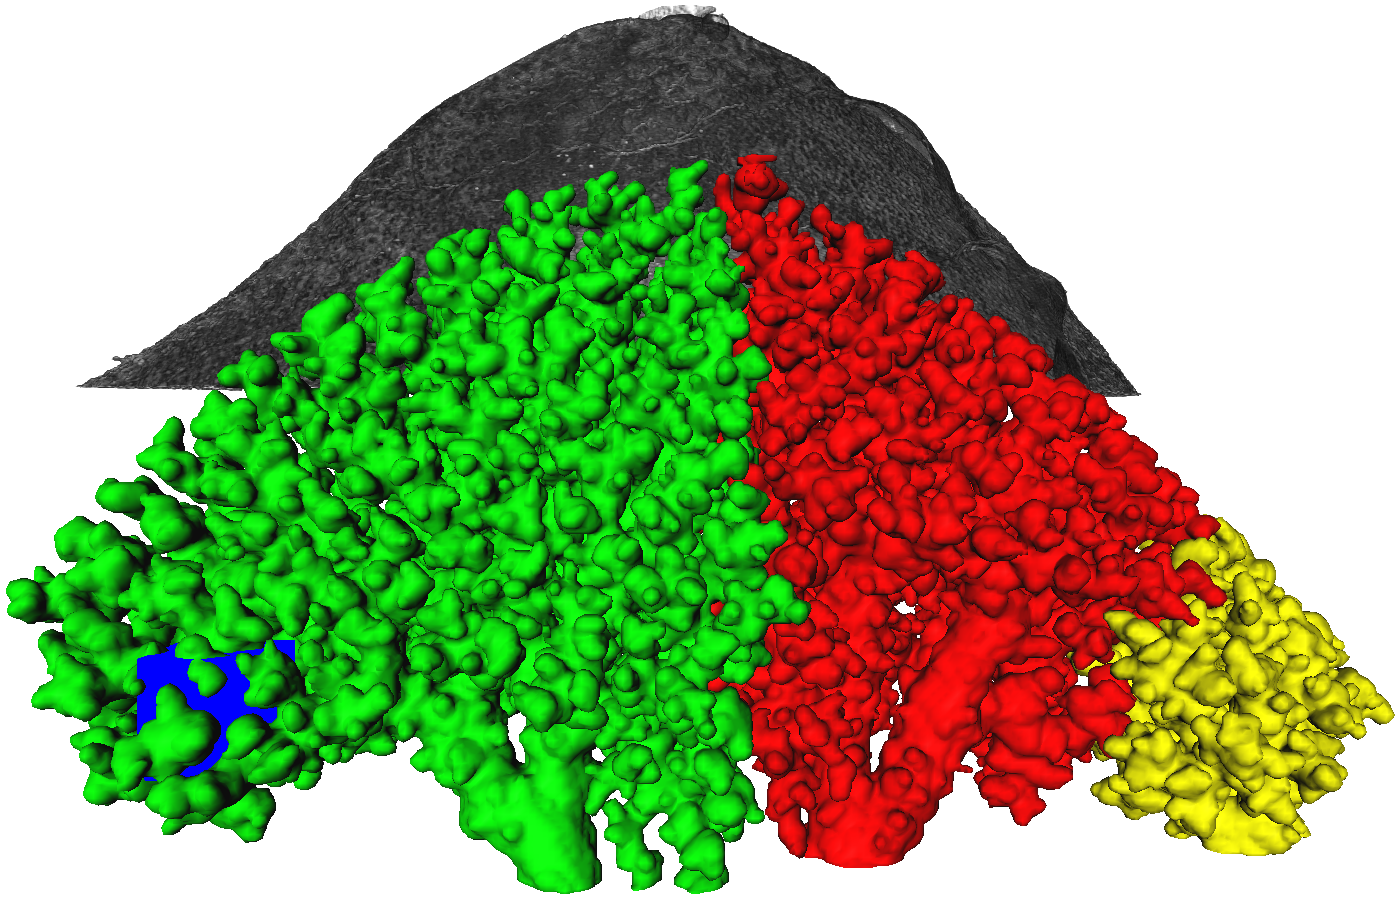
\includegraphics[width=\imagewidth]{img/comparisonBvsT/overview-t}};
				% 1391px = 4.0138mm > 100px = 288um > 173px = 500um
				\draw[|-|,thick] (6,774) -- (1395,839) node [sloped,midway,above] {\SI{4.0138}{\milli\meter}};
				\draw[|-|,thick] (\x,\y) -- (\x+173,\y) node [midway,above] {\SI{500}{\micro\meter}};
			\end{tikzpicture}%
			}\\%
		\pgfmathsetlength{\imagescale}{\imagewidth/806} % pixel width of imagefile used
		\def\x{345}
		\def\y{780}
		\subfloat[ROI inside green segment for protocol B]{%
			\label{subfig:DetailROIB}%
			\begin{tikzpicture}[x=\imagescale,y=-\imagescale]
				\node[anchor=north west,inner sep=0pt,outer sep=0pt] at (0,0)
					{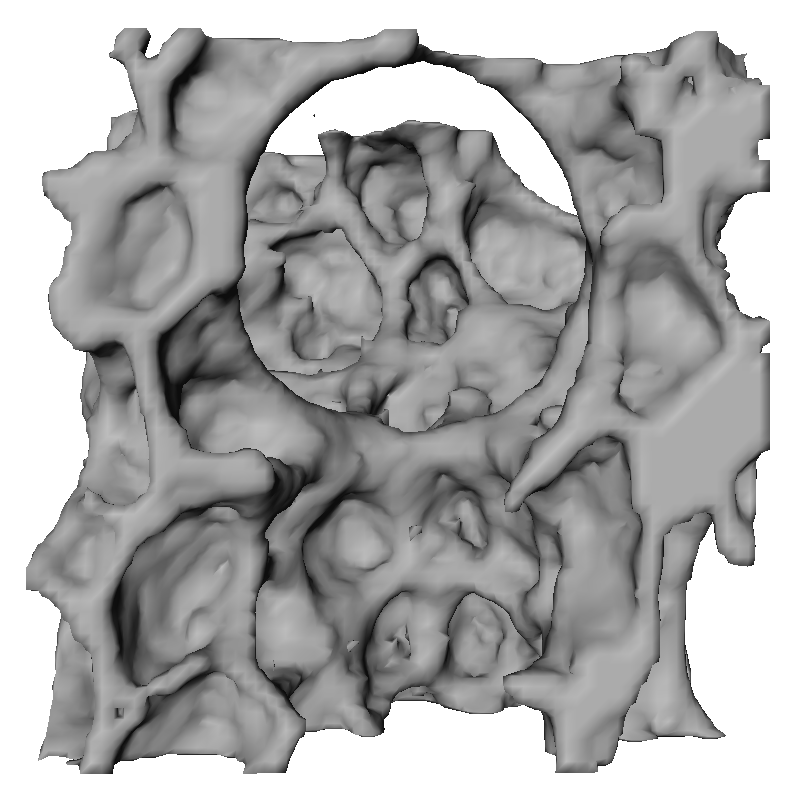
\includegraphics[width=\imagewidth]{img/comparisonBvsT/roi-b-nomedian}};
				% 746px = 0.18944mm > 100px = 25um > 196.9px = 50um
				\draw[|-|,thick] (27,270) -- (773,272) node [sloped,midway,above] {\SI{189.44}{\micro\meter}};
				\draw[|-|,thick] (\x,\y) -- (\x+196.9,\y) node [midway,above] {\SI{50}{\micro\meter}};
			\end{tikzpicture}%
			}%
		\subfloat[ROI inside green segment for protocol T]{%
			\label{subfig:DetailROIT}%
			\begin{tikzpicture}[x=\imagescale,y=-\imagescale]
				\node[anchor=north west,inner sep=0pt,outer sep=0pt] at (0,0)
					{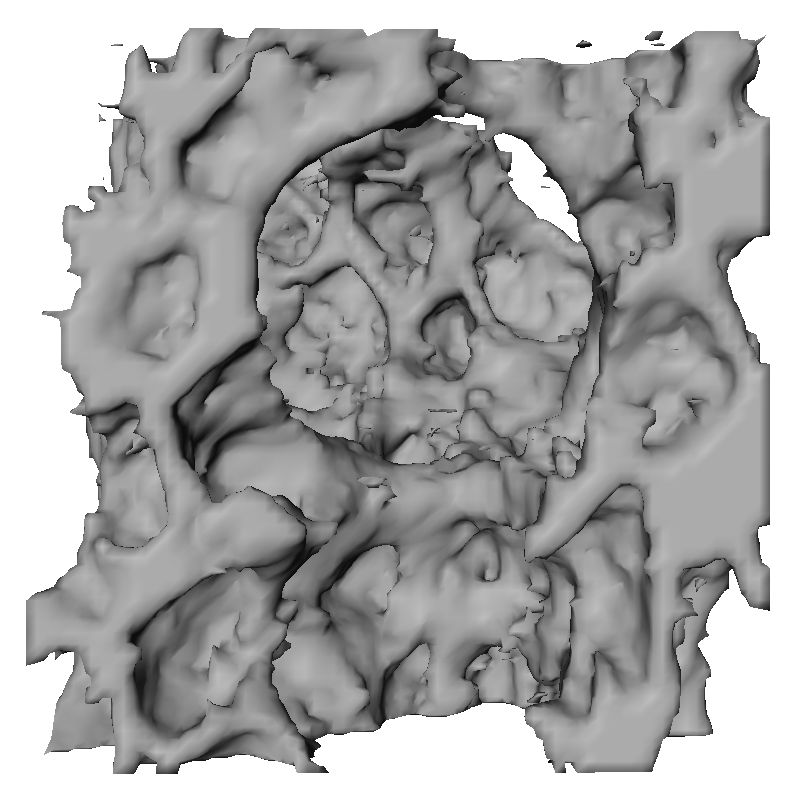
\includegraphics[width=\imagewidth]{img/comparisonBvsT/roi-t-nomedian}};
				% 744px = 0.18944mm > 100px = 25um > 196.5px = 50um
				\draw[|-|,thick] (27,311) -- (771,311) node [sloped,midway,above] {\SI{189.44}{\micro\meter}};
				\draw[|-|,thick] (\x,\y) -- (\x+196.5,\y) node [midway,above] {\SI{50}{\micro\meter}};
			\end{tikzpicture}%
			}%\\%
		%\subfloat[Detail B, median filtered ($3\times3\times3$)]{%
		%	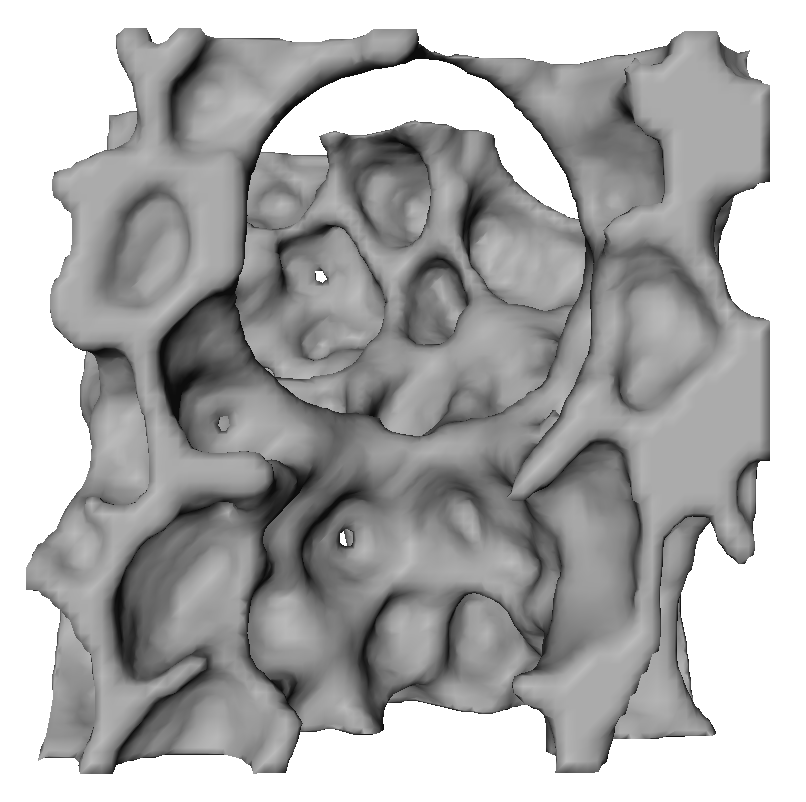
\includegraphics[width=\imsize]{img/comparisonBvsT/roi-b}%
		%	}%
		%\subfloat[Detail T, median filtered ($3\times3\times3$)]{%
		%	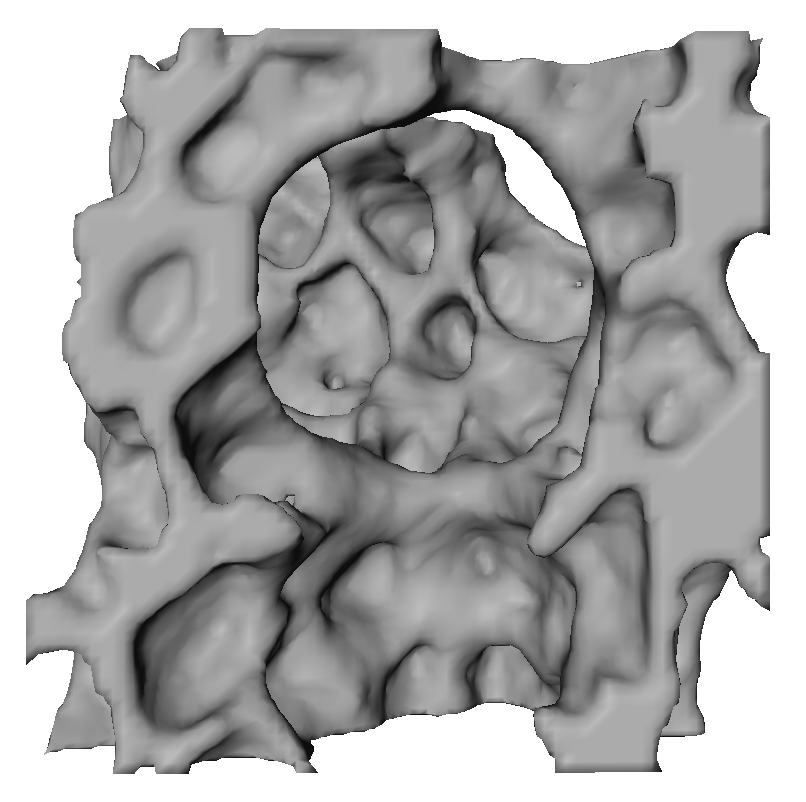
\includegraphics[width=\imsize]{img/comparisonBvsT/roi-t}%
		%	}%
	%	\caption[Comparison of 3D visualizations of protocols B and T]
		\caption{Comparison of three-dimensional visualizations of protocols B and T. Top: Three independent airway segments (green, red, yellow) have been extracted using a region growing algorithm. A cubical region of interest (ROI, blue) with a side length of 128 pixels (corresponding to \SI{190}{\micro\meter}) is marked inside the leftmost segment for both protocols. Bottom: Detailed view of isosurfaces of the lung tissue inside the ROIs shown above. Note the artifacts in the reconstructions for protocol T in subfigure~\subref{subfig:DetailROIT}.}%
		\label{fig:BvsT}%
	\end{figure*}
\fi

The field of view can be increased even further; we also scanned and reconstructed a rat lung sample with 5 scanning positions, resulting in a five-fold (4.74$\times$) increase in available field of view from 1024$\times$1024 pixels to 4850$\times$4851.5 pixels (see figure~\ref{fig:LungSlabSophie}). We have been able to reconstruct a sample with size of approximately 0.82$\times$7.18$\times$\SI{1.52}{\milli\meter} at a voxel side length of \SI{1.48}{\micro\meter}, see figure~\ref{fig:LungSlabSophie}.

\ifiucr
	%\onecolumn
	\begin{figure}%
		\centering%
		\caption{Visualization of lung tissue slab. %
				a): Three dimensional volume rendering of slab of lung tissue with a size of 554$\times$4854$\times$1024 pixels at a voxel side length of \SI{0.73}{\micro\meter}. Both inset cubes have a side length of 256 pixels and were automatically segmented using a region growing algorithm. %
				b): Close-up of inset cube at an outer position in the sample, including the background tissue. % 
				c): Close-up of inset cube at an outer position in the sample. Albeit we have been able to automatically segment the lung tissue, segmentation artifacts are visible. Single alveoli can be distinguished. %
				d): Close-up of inset cube at a central position in the sample. Single alveoli are clearly visible. %
				e): Close-up of inset cube at a central position in the sample, including the background tissue.%
		 		}%
		\renewcommand{\imsize}{\linewidth}%
		\pgfmathsetlength{\imagewidth}{\imsize}%
		\pgfmathsetlength{\imagescale}{\imagewidth/1589}%
		\begin{tikzpicture}[x=\imagescale,y=-\imagescale]%
			\def\x{1082}% scalebar-x at golden ratio
			\def\y{555}% scalebar-y at 90% of height
			\node[anchor=north west,inner sep=0pt,outer sep=0pt] at (0,0)%
				{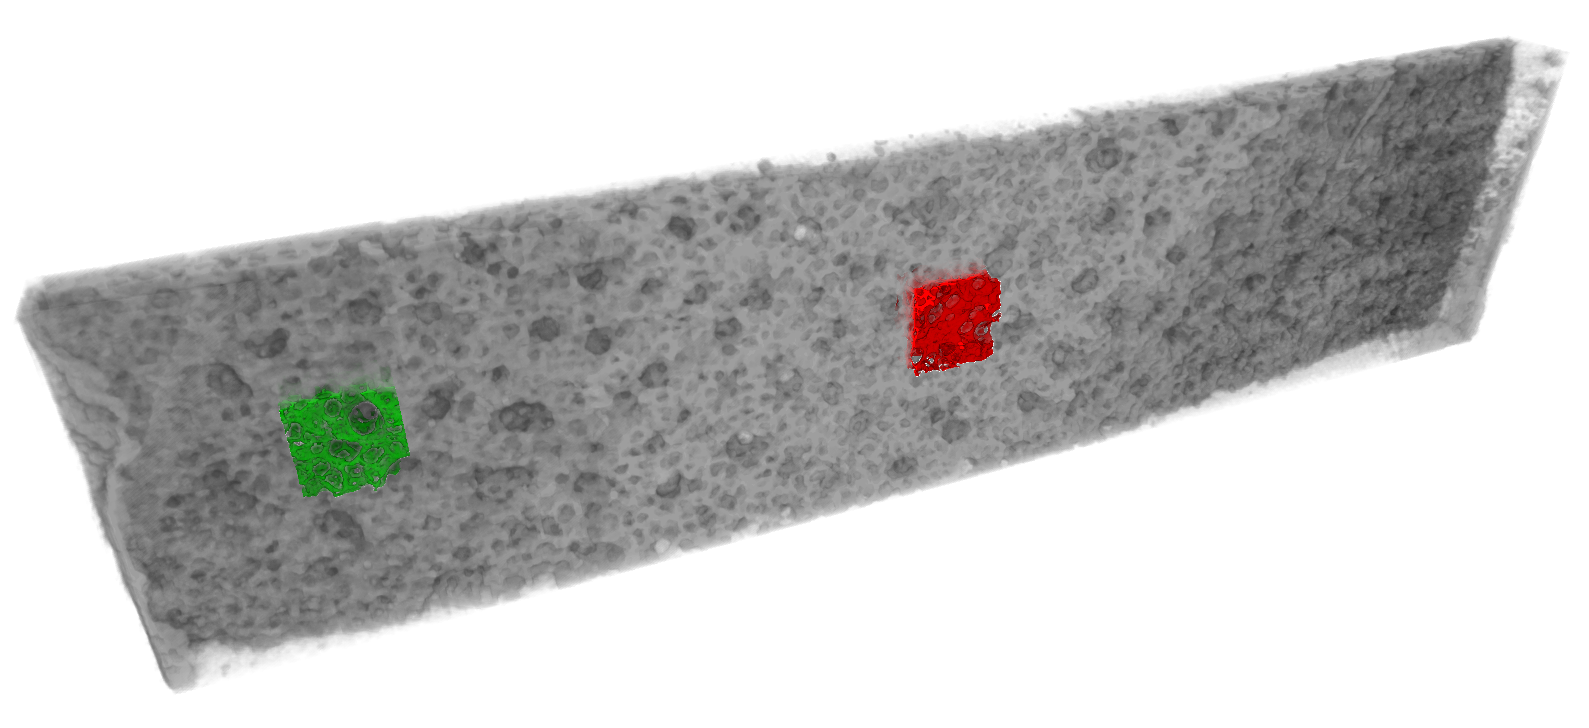
\includegraphics[width=\imagewidth]{img/sophie/full.png}};%
			\draw[|-|,thick] (17,319) -- (1568,58) node [sloped,midway,above] {\SI{7}{\milli\meter}};%
			\draw[|-|,thick] (\x,\y) -- (\x+219,\y) node [midway,above] {\SI{1}{\milli\meter}};%
			\node [anchor=south west] at (0,728) {a)};%
		\end{tikzpicture}%
		\\%
		\renewcommand{\imsize}{.25\linewidth}%
		\pgfmathsetlength{\imagewidth}{\imsize}% desired displayed width of image
		\pgfmathsetlength{\imagescale}{\imagewidth/902}% 1543*928 = width of imagefile used below
		\def\x{557}%
		\def\y{812}%
		\begin{tikzpicture}[x=\imagescale,y=-\imagescale]%
			\node[anchor=north west,inner sep=0pt,outer sep=0pt] at (0,0)%
				{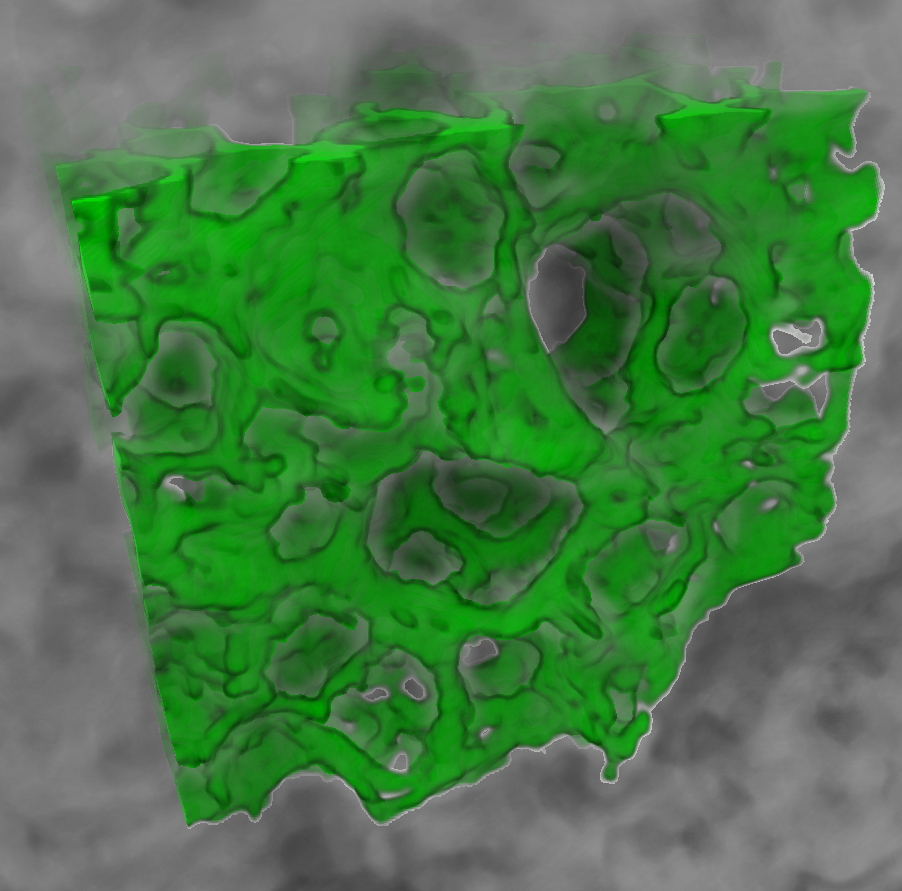
\includegraphics[width=\imagewidth]{img/sophie/crop-green-background}};%
			% 801px = 0.18944mm > 100px = 24um > 211.4px = 50um
			\draw[|-|,thick] (73,208) -- (866,93) node [sloped,midway,above] {\SI{0.18944}{\milli\meter}};%
			\draw[|-|,thick] (\x,\y) -- (\x+211.4,\y) node [midway,above] {\SI{50}{\micro\meter}};%
			\node [anchor=south west] at (0,891) {b)};%
		\end{tikzpicture}%
		\pgfmathsetlength{\imagewidth}{\imsize}% desired displayed width of image
		\pgfmathsetlength{\imagescale}{\imagewidth/902}% 1543*928 = width of imagefile used below
		\def\x{557}%
		\def\y{812}%
		\begin{tikzpicture}[x=\imagescale,y=-\imagescale]
			\node[anchor=north west,inner sep=0pt,outer sep=0pt] at (0,0)%
				{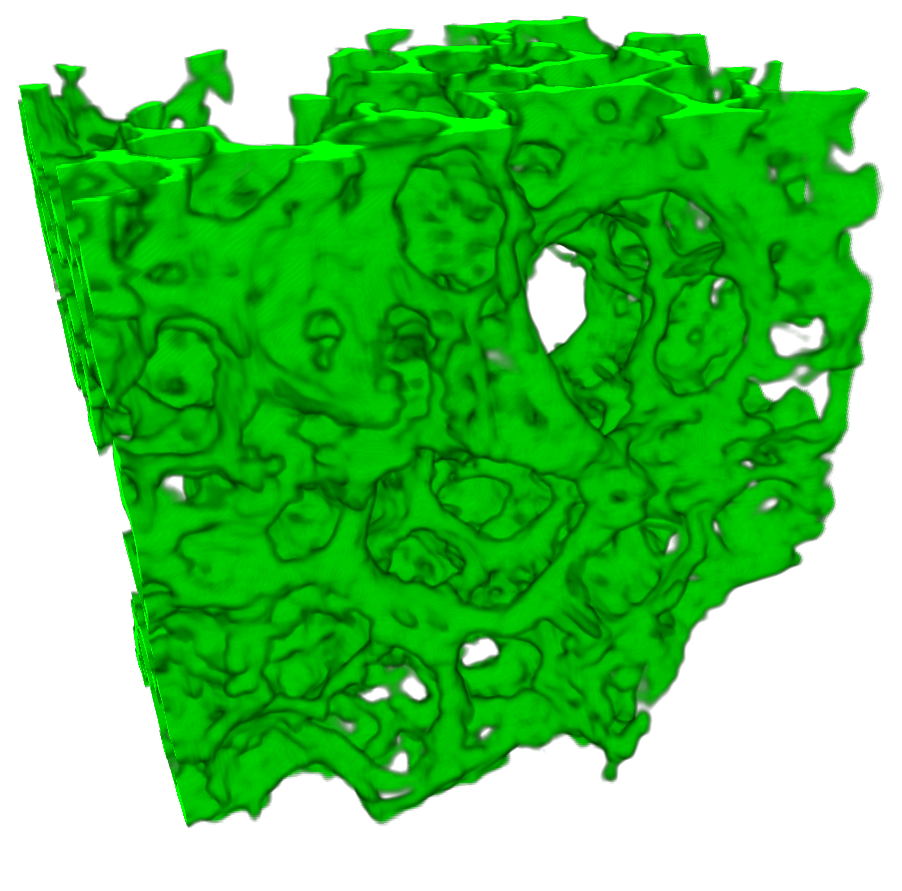
\includegraphics[width=\imagewidth]{img/sophie/crop-green}};%
			% 801px = 0.18944mm > 100px = 24um > 211.4px = 50um
			\draw[|-|,thick] (73,208) -- (866,93) node [sloped,midway,above] {\SI{0.18944}{\milli\meter}};%
			\draw[|-|,thick] (\x,\y) -- (\x+211.4,\y) node [midway,above] {\SI{50}{\micro\meter}};%
			\node [anchor=south west] at (0,891) {c)};%
		\end{tikzpicture}%
		\pgfmathsetlength{\imagewidth}{\imsize}% desired displayed width of image
		\pgfmathsetlength{\imagescale}{\imagewidth/902}% 1543*928 = width of imagefile used below
		\def\x{557}%
		\def\y{812}%
		\begin{tikzpicture}[x=\imagescale,y=-\imagescale]%
		     \node[anchor=north west,inner sep=0pt,outer sep=0pt] at (0,0)%
		         {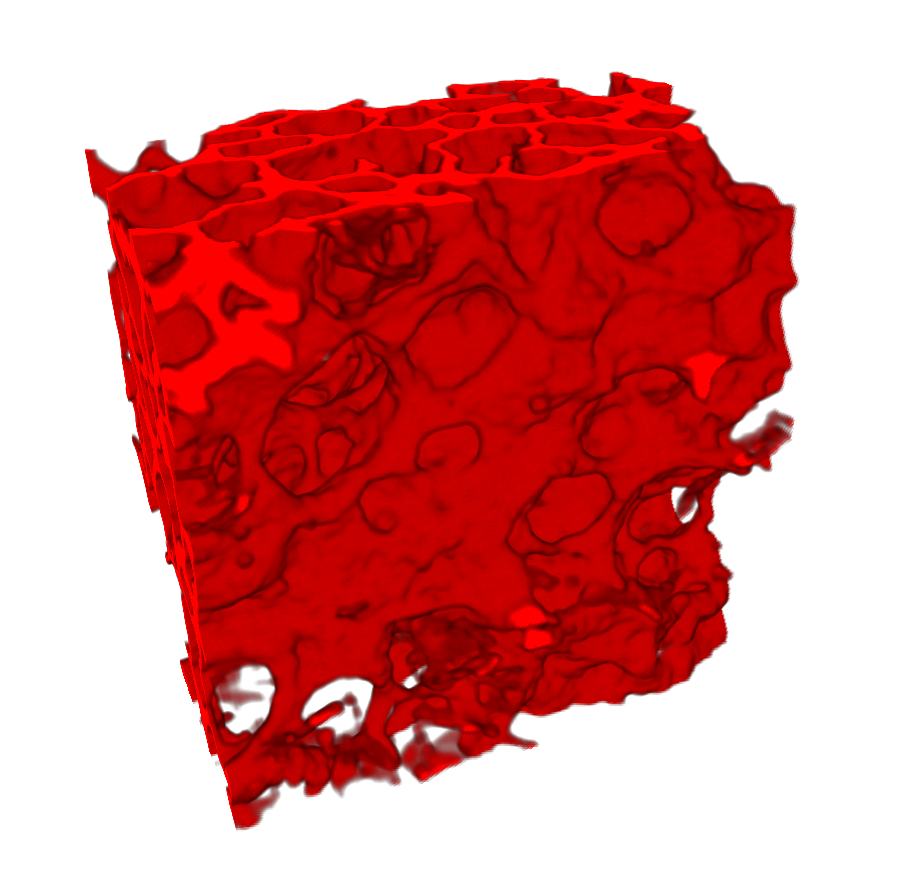
\includegraphics[width=\imagewidth]{img/sophie/crop-red}};%
			% 661px = 0.18944mm > 100px = 29um > 174.6px = 50um
			\draw[|-|,thick] (85,151) -- (741,66) node [sloped,midway,above] {\SI{189.44}{\micro\meter}};%
			\draw[|-|,thick] (\x,\y) -- (\x+174.6,\y) node [midway,above] {\SI{50}{\micro\meter}};%
			\node [anchor=south west] at (0,891) {d)};%
		\end{tikzpicture}%
		\pgfmathsetlength{\imagewidth}{\imsize}% desired displayed width of image
		\pgfmathsetlength{\imagescale}{\imagewidth/902}% 1543*928 = width of imagefile used below
		\def\x{557}%
		\def\y{812}%
		\begin{tikzpicture}[x=\imagescale,y=-\imagescale]%
		     \node[anchor=north west,inner sep=0pt,outer sep=0pt] at (0,0)%
		         {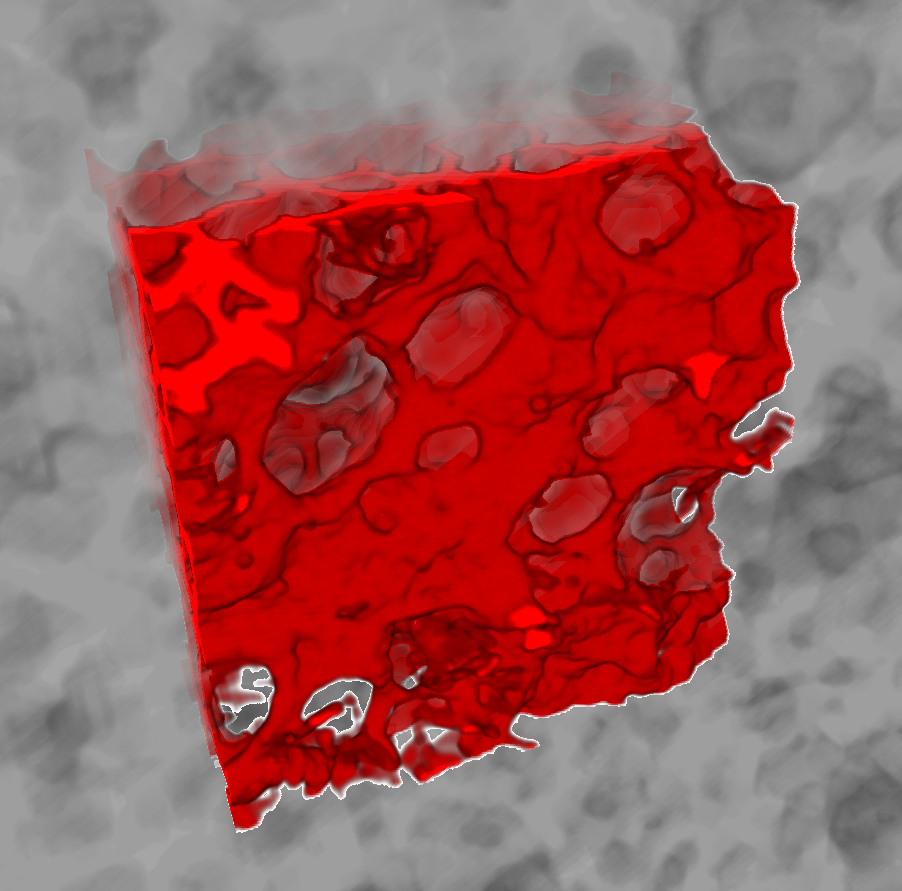
\includegraphics[width=\imagewidth]{img/sophie/crop-red-background}};%
			% 661px = 0.18944mm > 100px = 29um > 174.6px = 50um
			\draw[|-|,thick] (85,151) -- (741,66) node [sloped,midway,above] {\SI{189.44}{\micro\meter}};%
			\draw[|-|,thick] (\x,\y) -- (\x+174.6,\y) node [midway,above] {\SI{50}{\micro\meter}};%
			\node [anchor=south west] at (0,891) {e)};%
		\end{tikzpicture}%
		\label{fig:LungSlabSophie}%
	\end{figure}%
%\twocolumn
\else
	\begin{figure*}[htp]
		\renewcommand{\imsize}{\linewidth}%
		\pgfmathsetlength{\imagewidth}{\imsize} 		 % desired displayed width of image
		\pgfmathsetlength{\imagescale}{\imagewidth/1589} % 1589*728 = width of imagefile used below
		\centering
		\subfloat[Volume Rendering of lung tissue slab, including two ROI]{%
			\begin{tikzpicture}[x=\imagescale,y=-\imagescale]
				\def\x{982} % scalebar-x at golden ratio
				\def\y{655} % scalebar-y at 90% of height
				\node[anchor=north west,inner sep=0pt,outer sep=0pt] at (0,0)
					{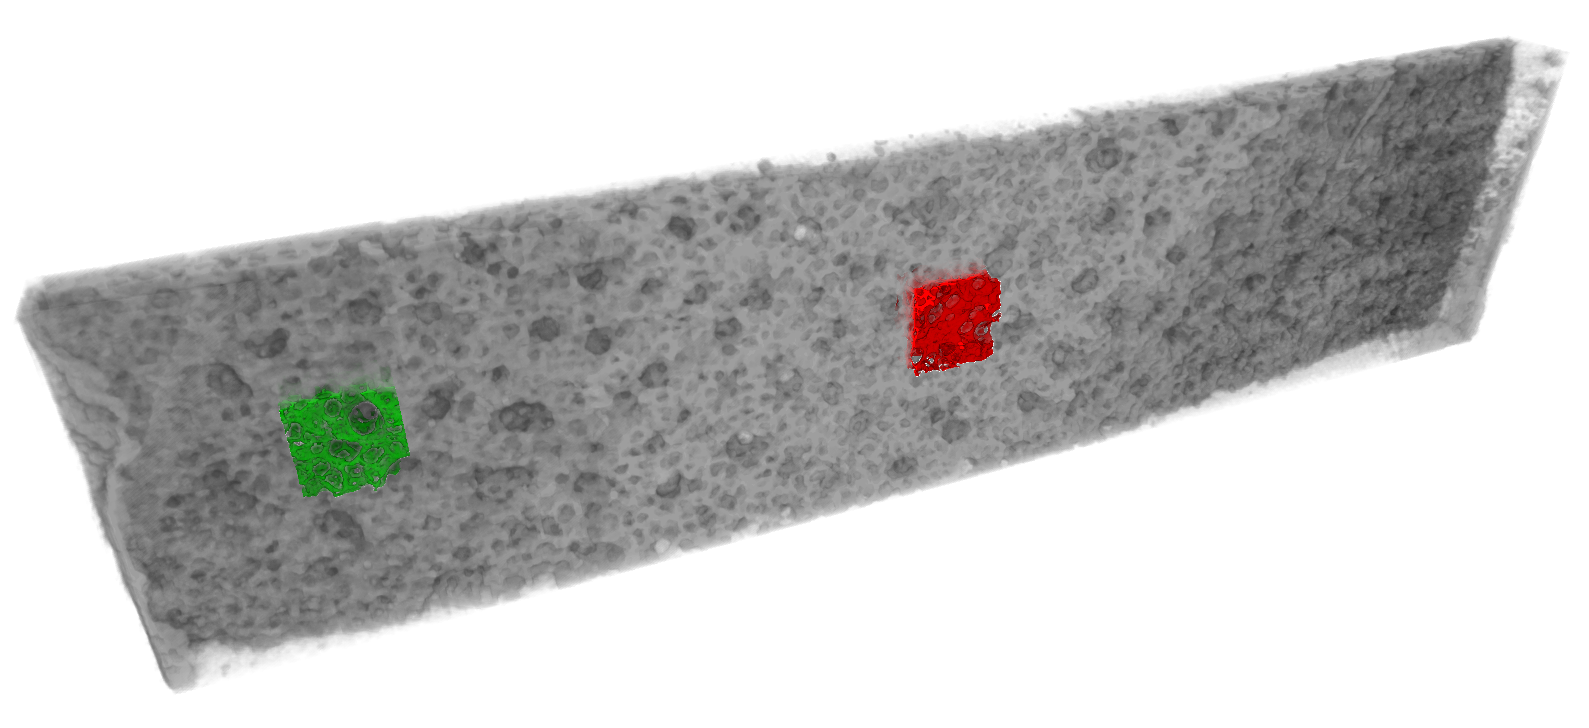
\includegraphics[width=\imagewidth]{img/sophie/full.png}};
				% 1572px = 3.592mm > 100px = 228um > 219px = 500um
				\draw[|-|,thick] (17,319) -- (1568,58) node [sloped,midway,above] {\SI{7}{\milli\meter}};
				\draw[|-|,thick] (\x,\y) -- (\x+219,\y) node [midway,above] {\SI{1}{\milli\meter}};
			\end{tikzpicture}%
			\label{subfig:LungSlab}%
			}%
		\renewcommand{\imsize}{.25\linewidth}
		\pgfmathsetlength{\imagewidth}{\imsize} % desired displayed width of image
		\pgfmathsetlength{\imagescale}{\imagewidth/902} % 1543*928 = width of imagefile used below
		\def\x{557}
		\def\y{812}
		\subfloat[ROI inside the lung tissue slab]{%
			\begin{tikzpicture}[x=\imagescale,y=-\imagescale]
				\node[anchor=north west,inner sep=0pt,outer sep=0pt] at (0,0)
					{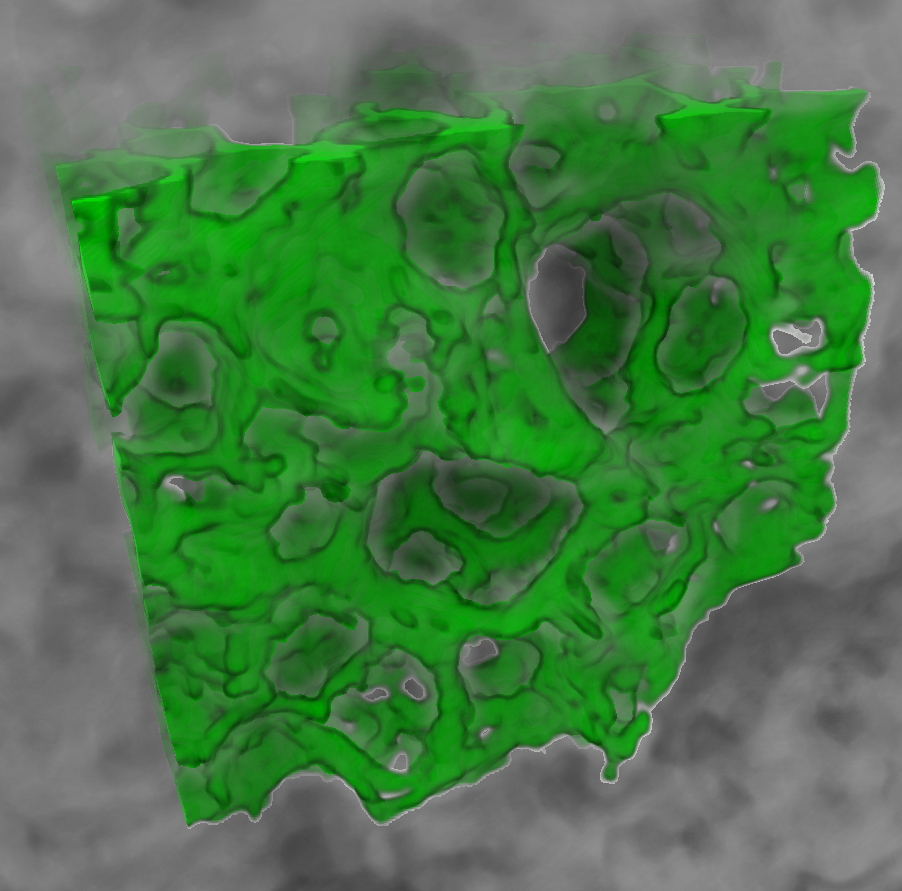
\includegraphics[width=\imagewidth]{img/sophie/crop-green-background}};
				% 801px = 0.18944mm > 100px = 24um > 211.4px = 50um
				\draw[|-|,thick] (73,208) -- (866,93) node [sloped,midway,above] {\SI{0.18944}{\milli\meter}};
				\draw[|-|,thick] (\x,\y) -- (\x+211.4,\y) node [midway,above] {\SI{50}{\micro\meter}};
			\end{tikzpicture}%
			\label{subfig:LungSlabDetailsGreenBG}%
			}%
		\subfloat[extracted ROI]{%
			\begin{tikzpicture}[x=\imagescale,y=-\imagescale]
				\node[anchor=north west,inner sep=0pt,outer sep=0pt] at (0,0)
					{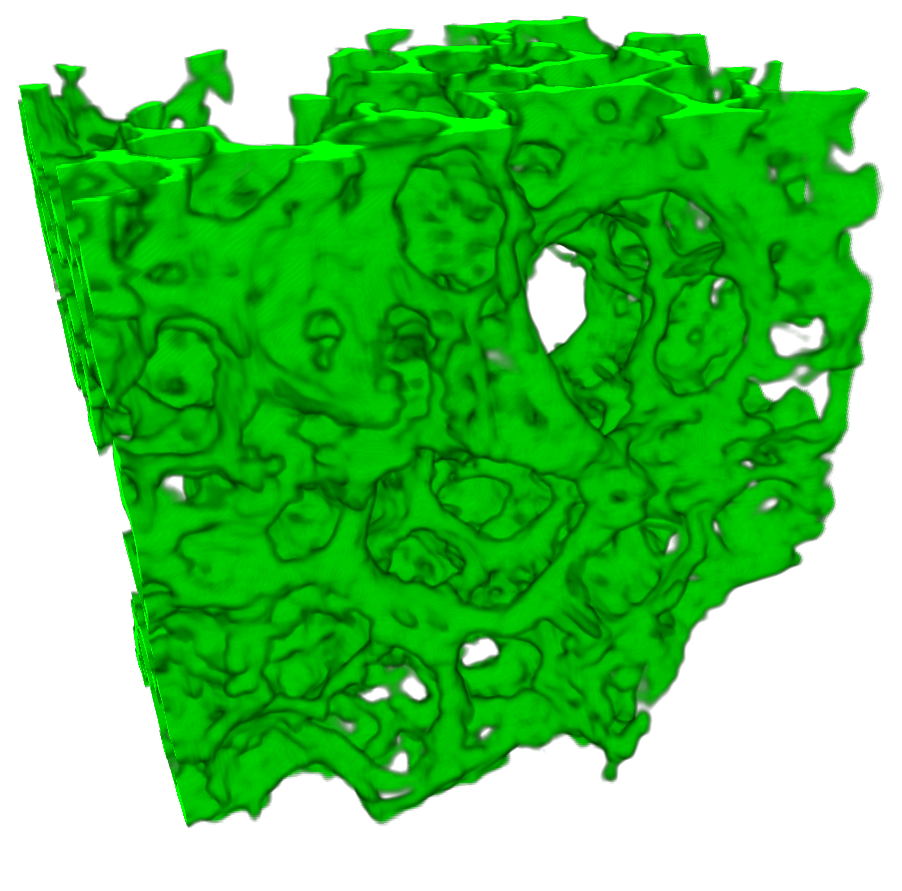
\includegraphics[width=\imagewidth]{img/sophie/crop-green}};
				% 801px = 0.18944mm > 100px = 24um > 211.4px = 50um
				\draw[|-|,thick] (73,208) -- (866,93) node [sloped,midway,above] {\SI{0.18944}{\milli\meter}};
				\draw[|-|,thick] (\x,\y) -- (\x+211.4,\y) node [midway,above] {\SI{50}{\micro\meter}};
			\end{tikzpicture}%
		 	\label{subfig:LungSlabDetailsGreen}%
			}%
		\subfloat[ROI inside the lung tissue slab]{%
			\begin{tikzpicture}[x=\imagescale,y=-\imagescale]
			     \node[anchor=north west,inner sep=0pt,outer sep=0pt] at (0,0)
			         {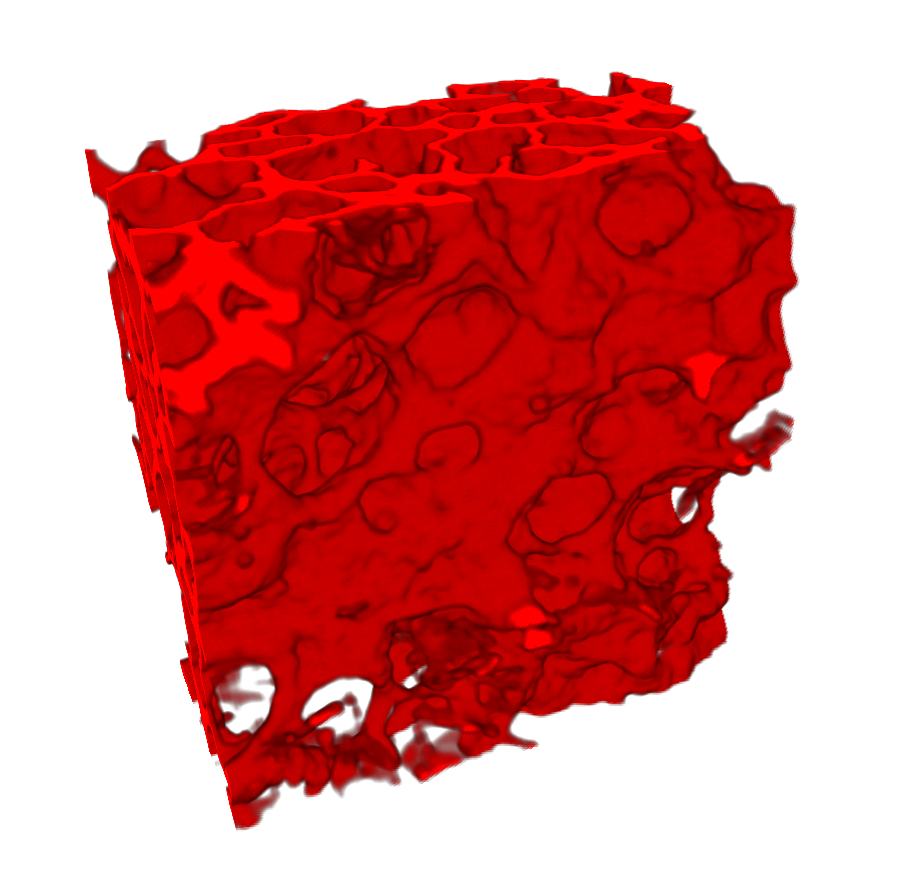
\includegraphics[width=\imagewidth]{img/sophie/crop-red}};
				% 661px = 0.18944mm > 100px = 29um > 174.6px = 50um
				\draw[|-|,thick] (85,151) -- (741,66) node [sloped,midway,above] {\SI{189.44}{\micro\meter}};
				\draw[|-|,thick] (\x,\y) -- (\x+174.6,\y) node [midway,above] {\SI{50}{\micro\meter}};
			\end{tikzpicture}%
			\label{subfig:LungSlabDetailsRed}%
			}%
		\subfloat[extracted ROI]{%
			\begin{tikzpicture}[x=\imagescale,y=-\imagescale]
			     \node[anchor=north west,inner sep=0pt,outer sep=0pt] at (0,0)
			         {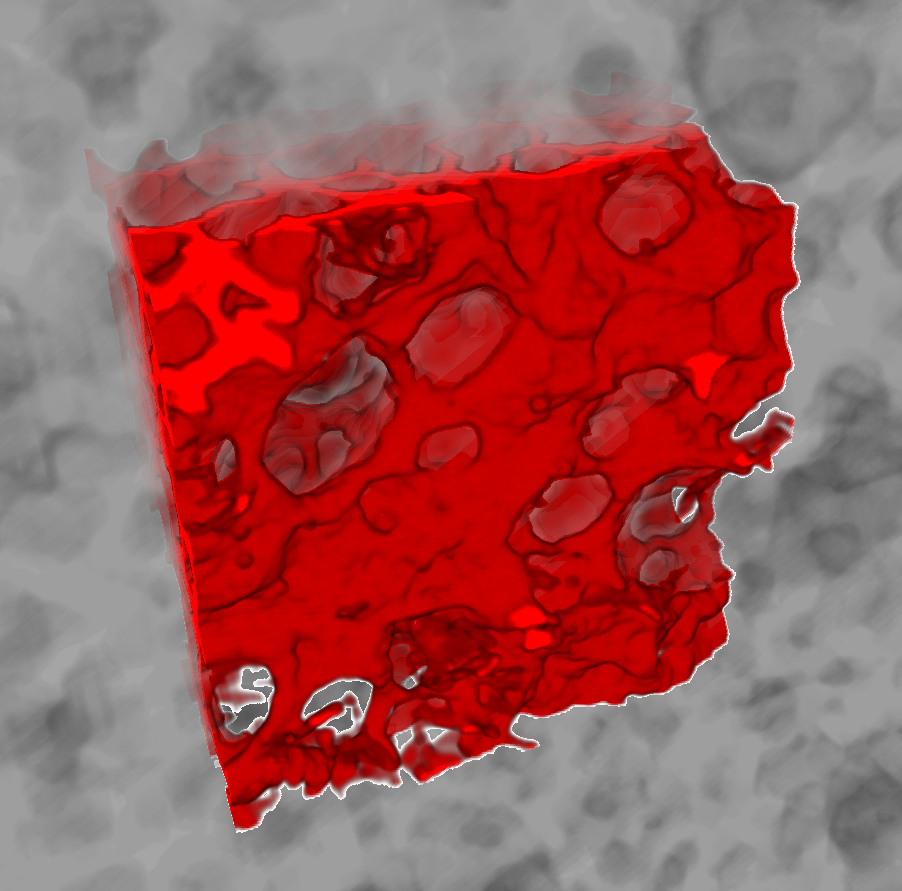
\includegraphics[width=\imagewidth]{img/sophie/crop-red-background}};
				% 661px = 0.18944mm > 100px = 29um > 174.6px = 50um
				\draw[|-|,thick] (85,151) -- (741,66) node [sloped,midway,above] {\SI{189.44}{\micro\meter}};
				\draw[|-|,thick] (\x,\y) -- (\x+174.6,\y) node [midway,above] {\SI{50}{\micro\meter}};
			\end{tikzpicture}%
		 	\label{subfig:LungSlabDetailsRedBG}%
			}%
	%	\caption[Visualization of lung tissue slab.]
		\caption{Visualization of lung tissue slab: %
			\subref{subfig:LungSlab}: Three dimensional volume rendering of slab of lung tissue with a size of 554$\times$4854$\times$1024 pixels at a voxel side length of \SI{0.14}{\micro\meter}. Both inset cubes have a side length of 128 pixels and were automatically segmented using a region growing algorithm. 
	 		\subref{subfig:LungSlabDetailsGreenBG}: Close-up of inset cube at an outer position in the sample, including the background tissue. % 
	 		\subref{subfig:LungSlabDetailsGreen}: Close-up of inset cube at an outer position in the sample. Albeit we have been able to automatically segment the lung tissue, segmentation artifacts are visible. Single alveoli can be distinguished. %
	 		\subref{subfig:LungSlabDetailsRed}: Close-up of inset cube at a central position in the sample. Single alveoli are clearly visible. %
	 		\subref{subfig:LungSlabDetailsRedBG}: Close-up of inset cube at a central position in the sample, including the background tissue.%
	 		}%
		\label{fig:LungSlabSophie}%
	\end{figure*}
	% normal figures %%%
\fi